\documentclass[12pt]{article}
\date{March 30, 2020}
\usepackage{pgf-pie}
\usepackage{pgfplots}
\usepackage{pgfplotstable}
\usetikzlibrary{patterns}
\usepackage[section]{placeins}
\usepackage[utf8]{inputenc}

\begin{document}


\clearpage{}
\section{Identification Number}

\label{sec:13}


\begin{figure}[h!]
    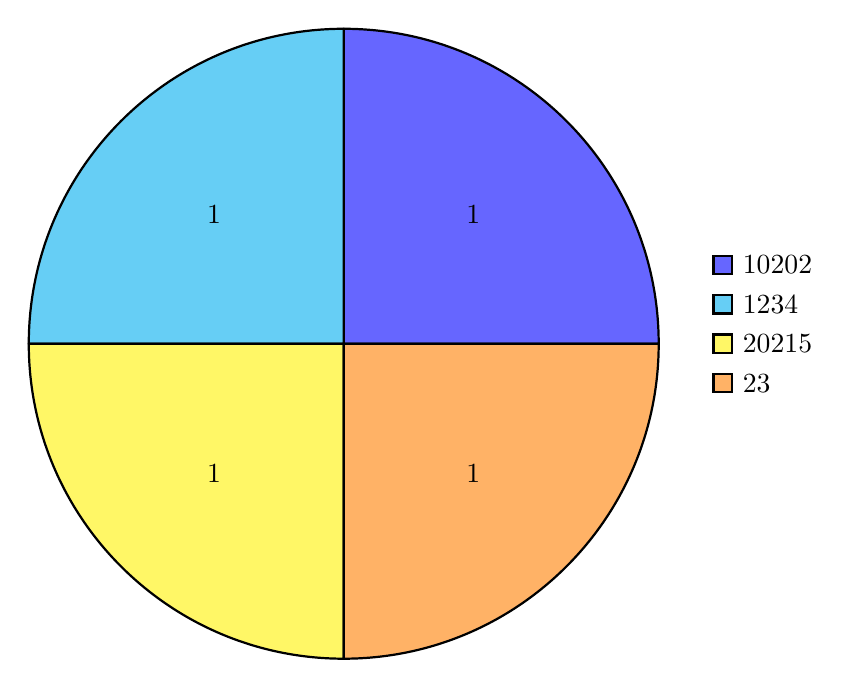
\begin{tikzpicture}
        \pie[radius=4,sum=auto,text=legend]{
            1/10202,
            1/1234,
            1/20215,
            1/23
        }
    \end{tikzpicture}
    \caption{\label{figure:q13-1}Repartition of answers for the question 'Identification Number'.}
\end{figure}



\clearpage{}
\section{18
Crown, Root, Treatment}

\label{sec:25}


\begin{figure}[h!]
    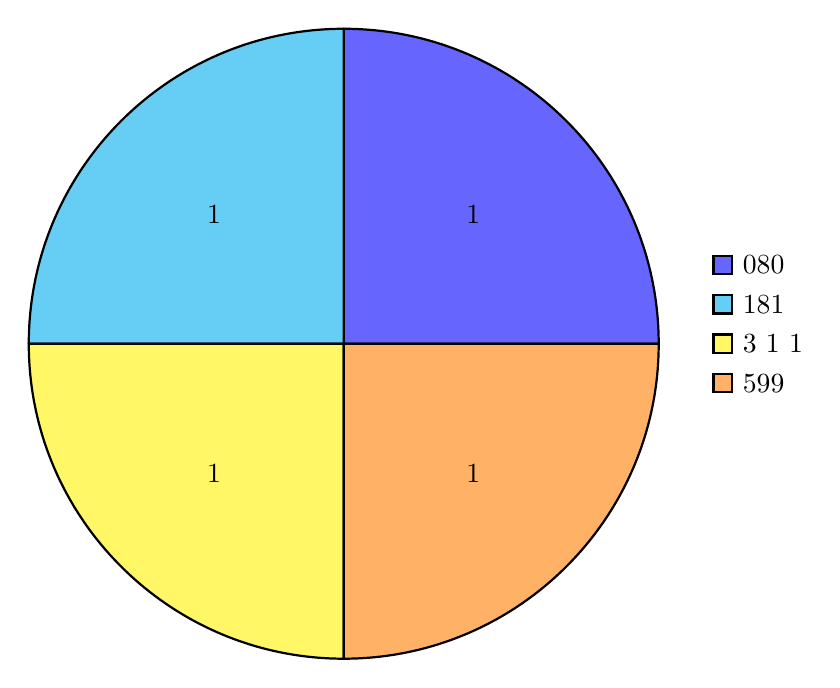
\begin{tikzpicture}
        \pie[radius=4,sum=auto,text=legend]{
            1/080,
            1/181,
            1/3 1 1,
            1/599
        }
    \end{tikzpicture}
    \caption{\label{figure:q25-1}Repartition of answers for the question '18
Crown, Root, Treatment'.}
\end{figure}



\clearpage{}
\section{Gingival Bleeding Scores
17/16 - B}

\label{sec:57}


\begin{figure}[h!]
    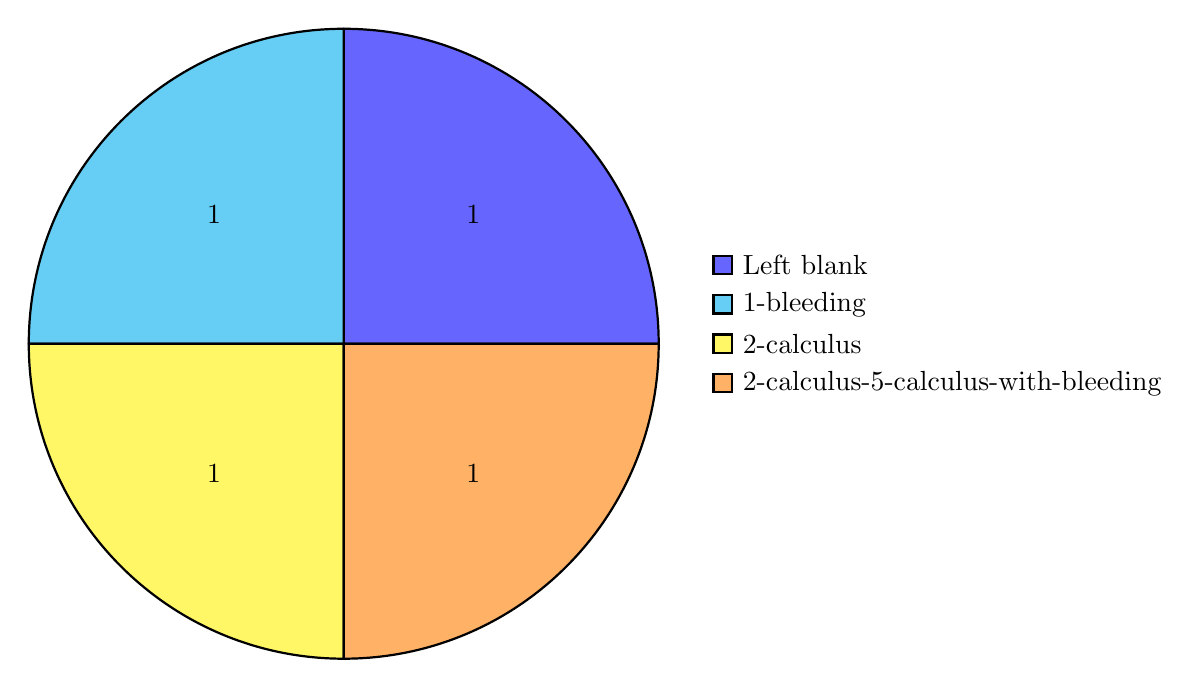
\begin{tikzpicture}
        \pie[radius=4,sum=auto,text=legend]{
            1/Left blank,
            1/1-bleeding,
            1/2-calculus,
            1/2-calculus-5-calculus-with-bleeding
        }
    \end{tikzpicture}
    \caption{\label{figure:q57-1}Repartition of answers for the question 'Gingival Bleeding Scores
17/16 - B'.}
\end{figure}



\clearpage{}
\section{Prosthetic Status
Upper}

\label{sec:69}


\begin{figure}[h!]
    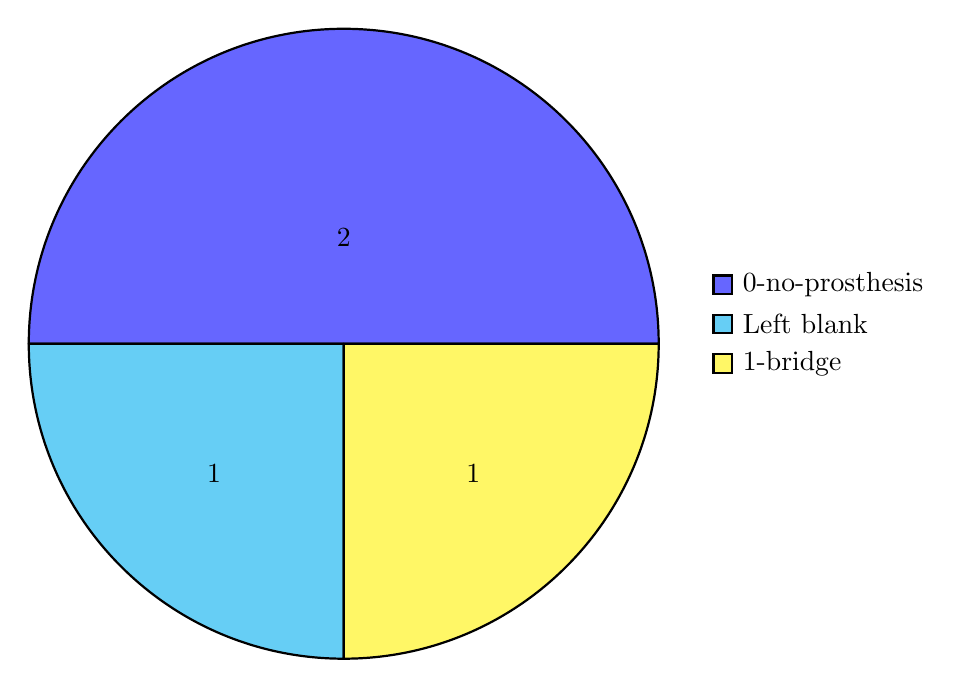
\begin{tikzpicture}
        \pie[radius=4,sum=auto,text=legend]{
            2/0-no-prosthesis,
            1/Left blank,
            1/1-bridge
        }
    \end{tikzpicture}
    \caption{\label{figure:q69-1}Repartition of answers for the question 'Prosthetic Status
Upper'.}
\end{figure}



\clearpage{}
\section{Clinical Condition}

\label{sec:168}


\begin{figure}[h!]
    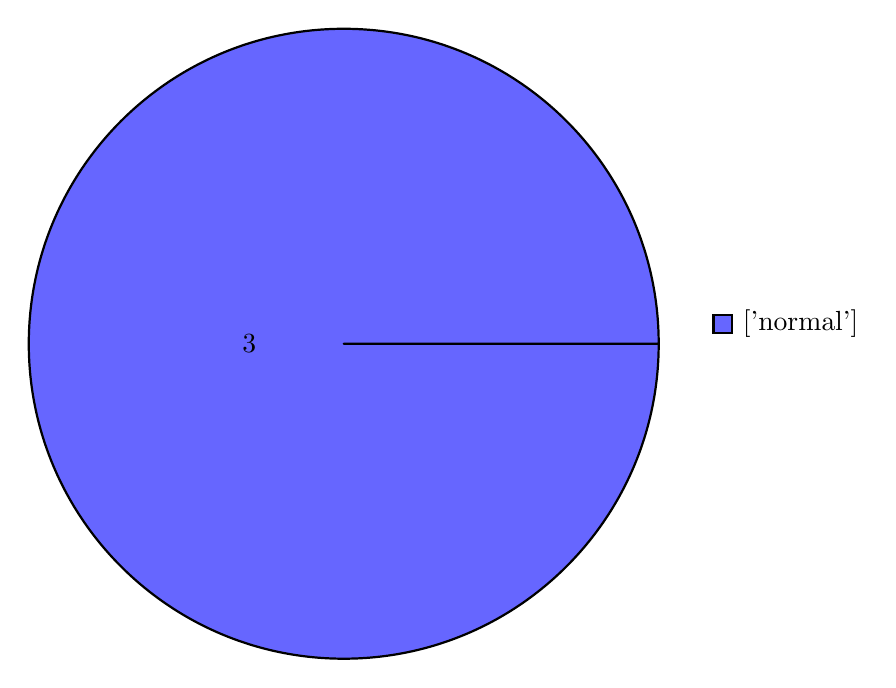
\begin{tikzpicture}
        \pie[radius=4,sum=auto,text=legend]{
            3/['normal']
        }
    \end{tikzpicture}
    \caption{\label{figure:q168-1}Repartition of answers for the question 'Clinical Condition'.}
\end{figure}



\clearpage{}
\section{Occlusal
Number of teeth affected}

\label{sec:174}


\begin{figure}[h!]
    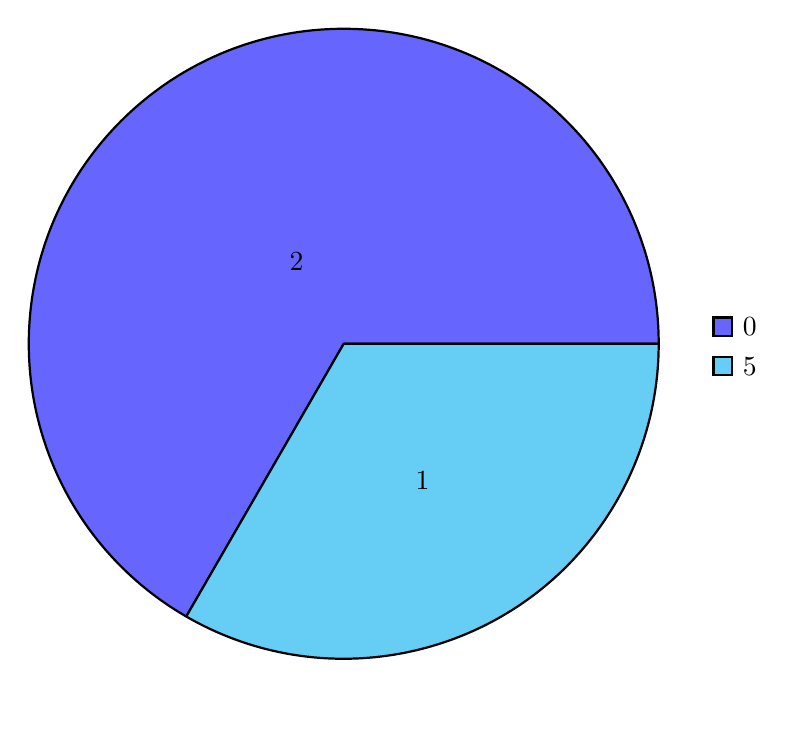
\begin{tikzpicture}
        \pie[radius=4,sum=auto,text=legend]{
            2/0,
            1/5
        }
    \end{tikzpicture}
    \caption{\label{figure:q174-1}Repartition of answers for the question 'Occlusal
Number of teeth affected'.}
\end{figure}



\clearpage{}
\section{Right}

\label{sec:247}


\begin{figure}[h!]
    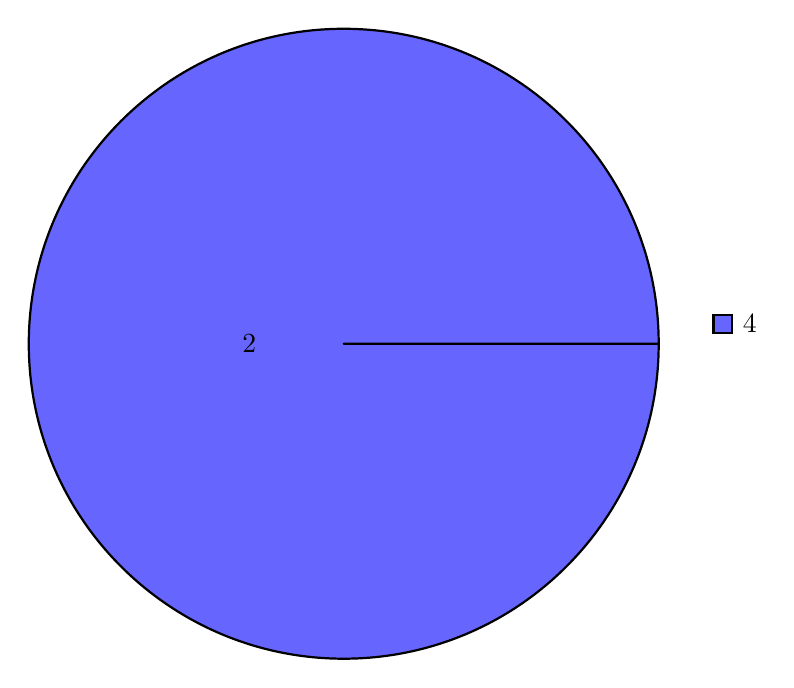
\begin{tikzpicture}
        \pie[radius=4,sum=auto,text=legend]{
            2/4
        }
    \end{tikzpicture}
    \caption{\label{figure:q247-1}Repartition of answers for the question 'Right'.}
\end{figure}



\clearpage{}
\section{17
Crown, Root, Treatment}

\label{sec:26}


\begin{figure}[h!]
    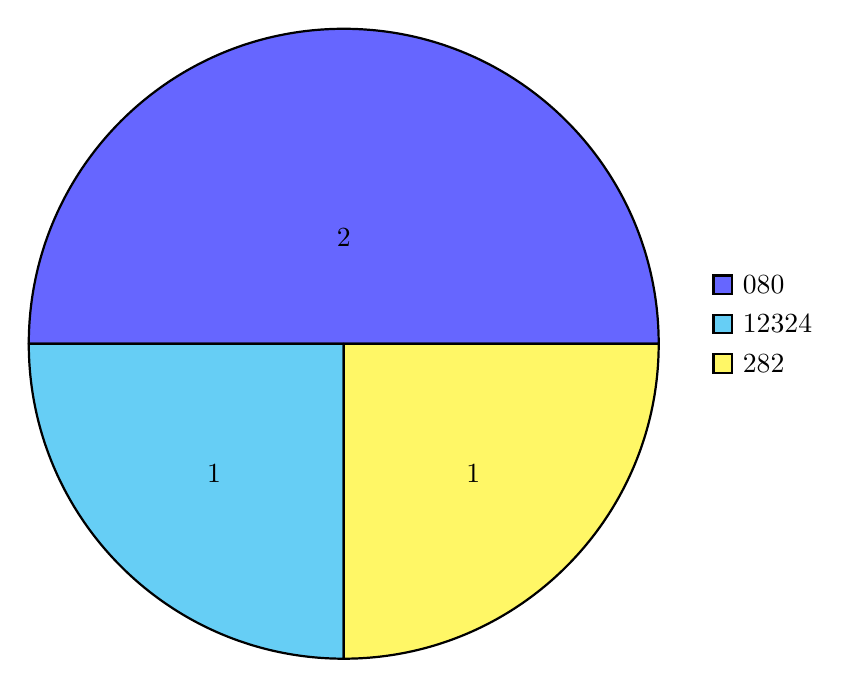
\begin{tikzpicture}
        \pie[radius=4,sum=auto,text=legend]{
            2/080,
            1/12324 ,
            1/282
        }
    \end{tikzpicture}
    \caption{\label{figure:q26-1}Repartition of answers for the question '17
Crown, Root, Treatment'.}
\end{figure}



\clearpage{}
\section{Gingival Bleeding Scores
11 - B}

\label{sec:59}


\begin{figure}[h!]
    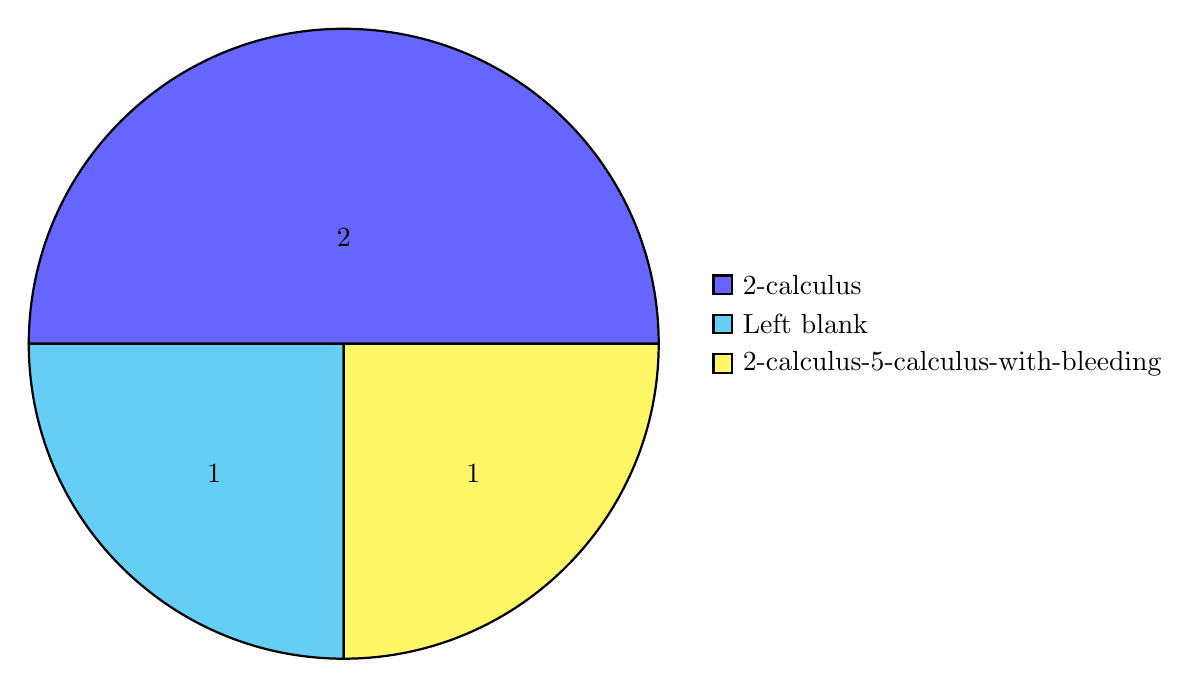
\begin{tikzpicture}
        \pie[radius=4,sum=auto,text=legend]{
            2/2-calculus,
            1/Left blank,
            1/2-calculus-5-calculus-with-bleeding
        }
    \end{tikzpicture}
    \caption{\label{figure:q59-1}Repartition of answers for the question 'Gingival Bleeding Scores
11 - B'.}
\end{figure}



\clearpage{}
\section{Prosthetic Status
Lower}

\label{sec:70}


\begin{figure}[h!]
    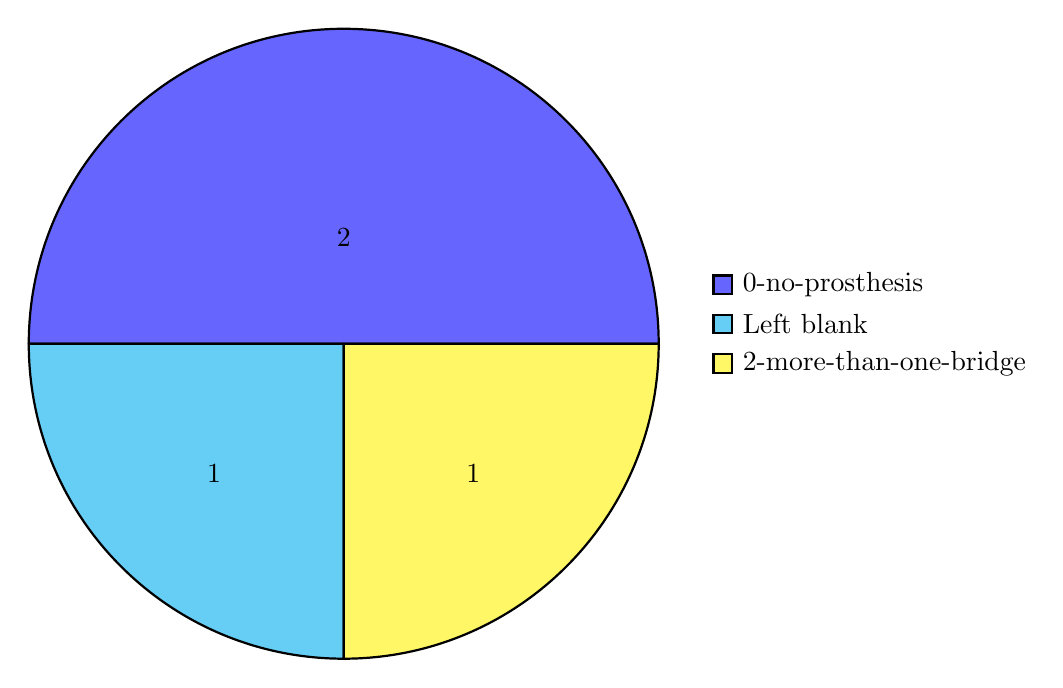
\begin{tikzpicture}
        \pie[radius=4,sum=auto,text=legend]{
            2/0-no-prosthesis,
            1/Left blank,
            1/2-more-than-one-bridge
        }
    \end{tikzpicture}
    \caption{\label{figure:q70-1}Repartition of answers for the question 'Prosthetic Status
Lower'.}
\end{figure}



\clearpage{}
\section{IF CONDITION Is White Lesion 
Location is}

\label{sec:169}


\begin{figure}[h!]
    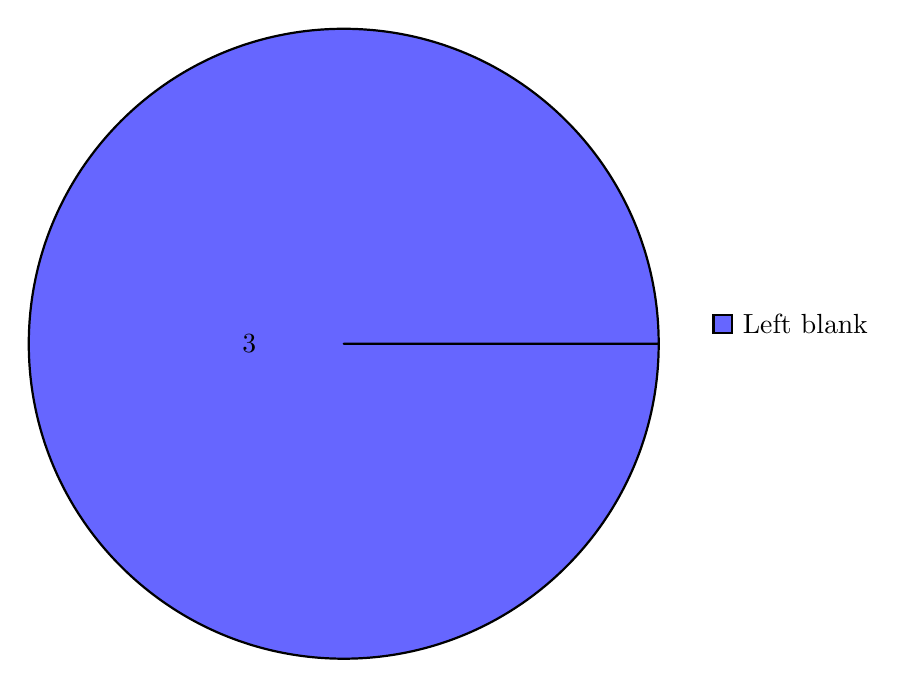
\begin{tikzpicture}
        \pie[radius=4,sum=auto,text=legend]{
            3/Left blank
        }
    \end{tikzpicture}
    \caption{\label{figure:q169-1}Repartition of answers for the question 'IF CONDITION Is White Lesion 
Location is'.}
\end{figure}



\clearpage{}
\section{Incisal
Number of teeth affected}

\label{sec:175}


\begin{figure}[h!]
    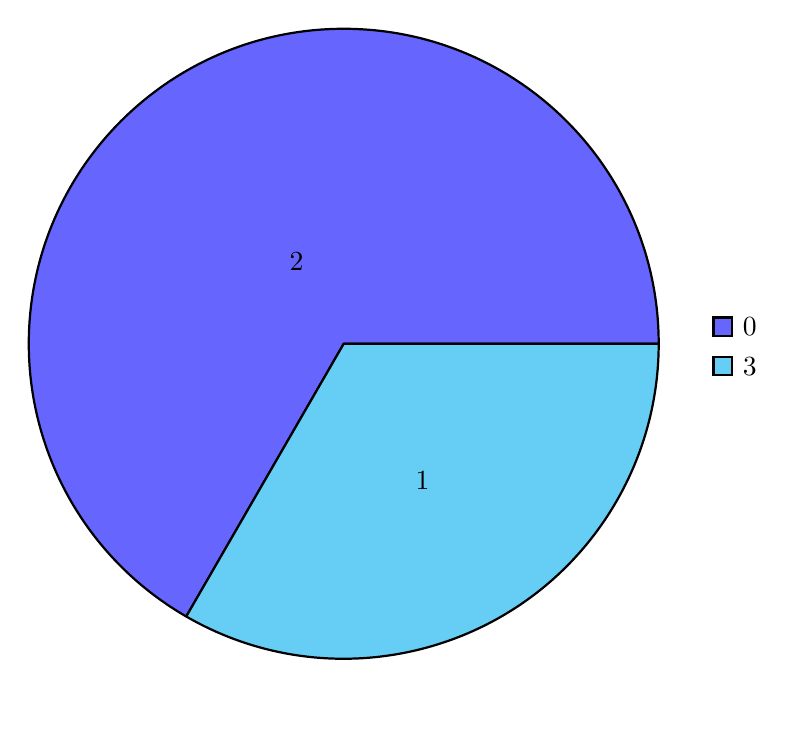
\begin{tikzpicture}
        \pie[radius=4,sum=auto,text=legend]{
            2/0,
            1/3
        }
    \end{tikzpicture}
    \caption{\label{figure:q175-1}Repartition of answers for the question 'Incisal
Number of teeth affected'.}
\end{figure}



\clearpage{}
\section{Left}

\label{sec:248}


\begin{figure}[h!]
    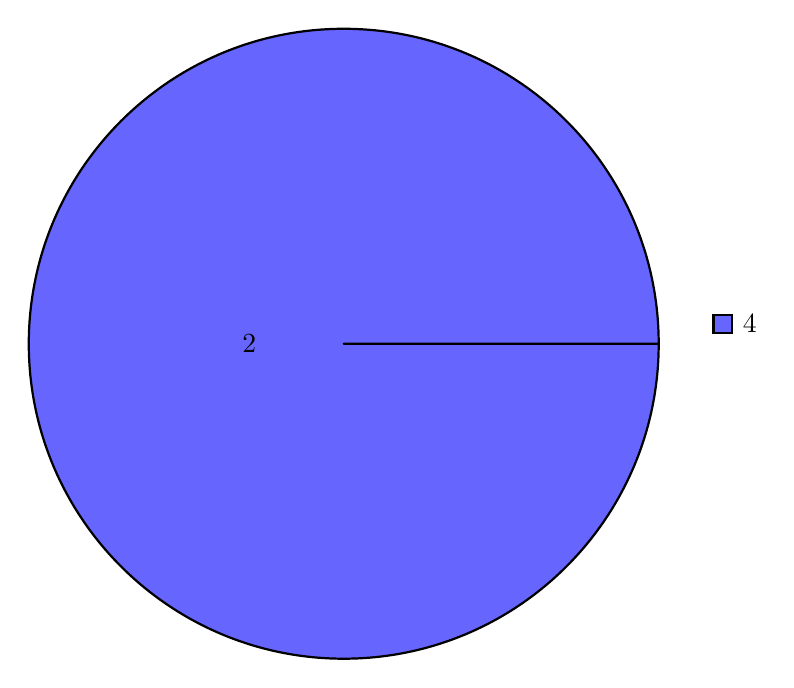
\begin{tikzpicture}
        \pie[radius=4,sum=auto,text=legend]{
            2/4
        }
    \end{tikzpicture}
    \caption{\label{figure:q248-1}Repartition of answers for the question 'Left'.}
\end{figure}



\clearpage{}
\section{Location Type}

\label{sec:15}


\begin{figure}[h!]
    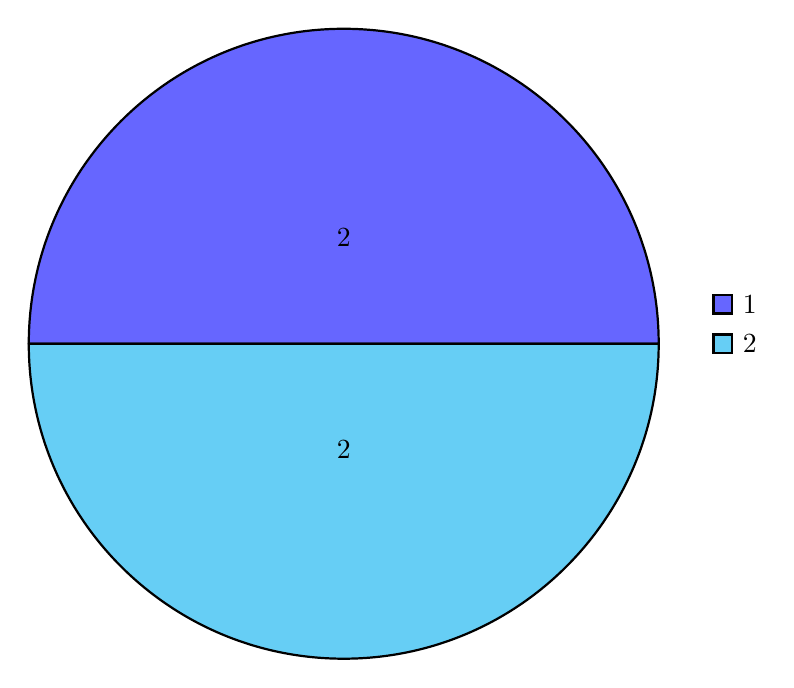
\begin{tikzpicture}
        \pie[radius=4,sum=auto,text=legend]{
            2/1,
            2/2
        }
    \end{tikzpicture}
    \caption{\label{figure:q15-1}Repartition of answers for the question 'Location Type'.}
\end{figure}



\clearpage{}
\section{16
Crown, Root, Treatment}

\label{sec:27}


\begin{figure}[h!]
    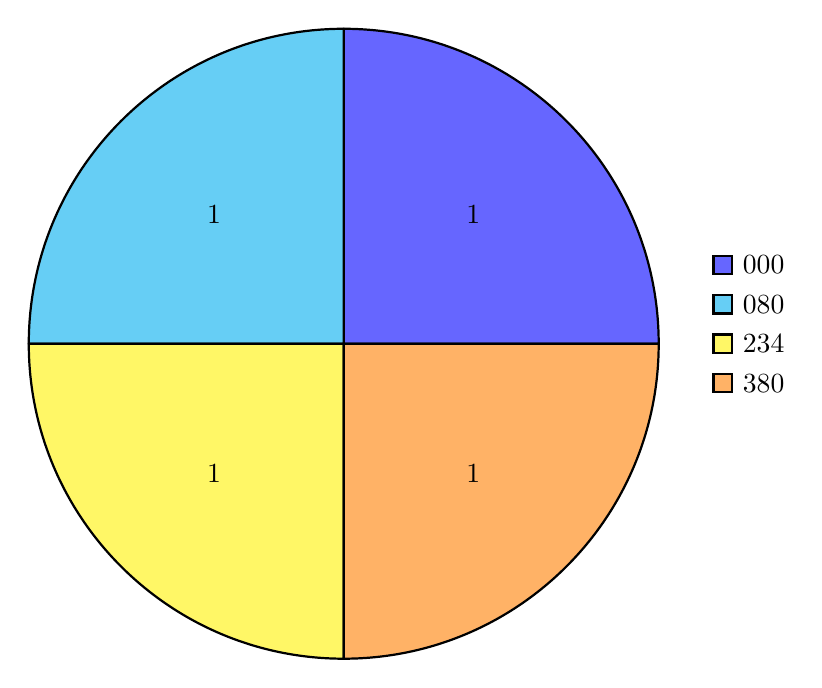
\begin{tikzpicture}
        \pie[radius=4,sum=auto,text=legend]{
            1/000,
            1/080,
            1/234 ,
            1/380
        }
    \end{tikzpicture}
    \caption{\label{figure:q27-1}Repartition of answers for the question '16
Crown, Root, Treatment'.}
\end{figure}



\clearpage{}
\section{Gingival Bleeding Scores
26/27 - B}

\label{sec:60}


\begin{figure}[h!]
    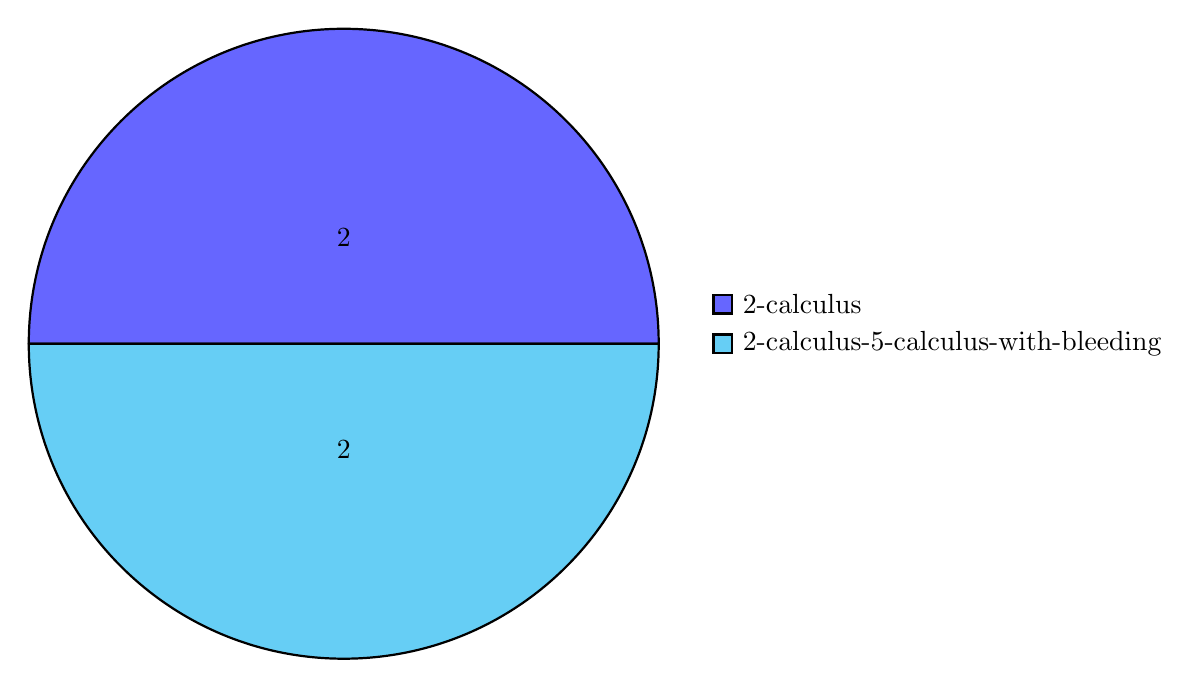
\begin{tikzpicture}
        \pie[radius=4,sum=auto,text=legend]{
            2/2-calculus,
            2/2-calculus-5-calculus-with-bleeding
        }
    \end{tikzpicture}
    \caption{\label{figure:q60-1}Repartition of answers for the question 'Gingival Bleeding Scores
26/27 - B'.}
\end{figure}



\clearpage{}
\section{Prosthetic Need
Upper}

\label{sec:71}


\begin{figure}[h!]
    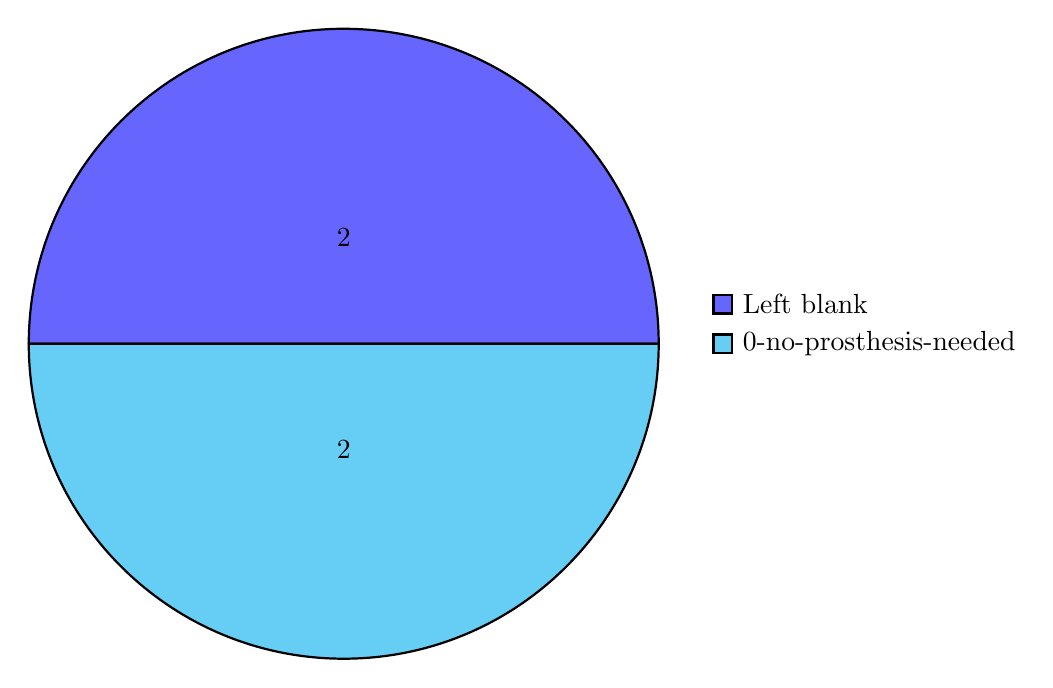
\begin{tikzpicture}
        \pie[radius=4,sum=auto,text=legend]{
            2/Left blank,
            2/0-no-prosthesis-needed
        }
    \end{tikzpicture}
    \caption{\label{figure:q71-1}Repartition of answers for the question 'Prosthetic Need
Upper'.}
\end{figure}



\clearpage{}
\section{IF CONDITION Is Red Lesion 
Location is}

\label{sec:170}


\begin{figure}[h!]
    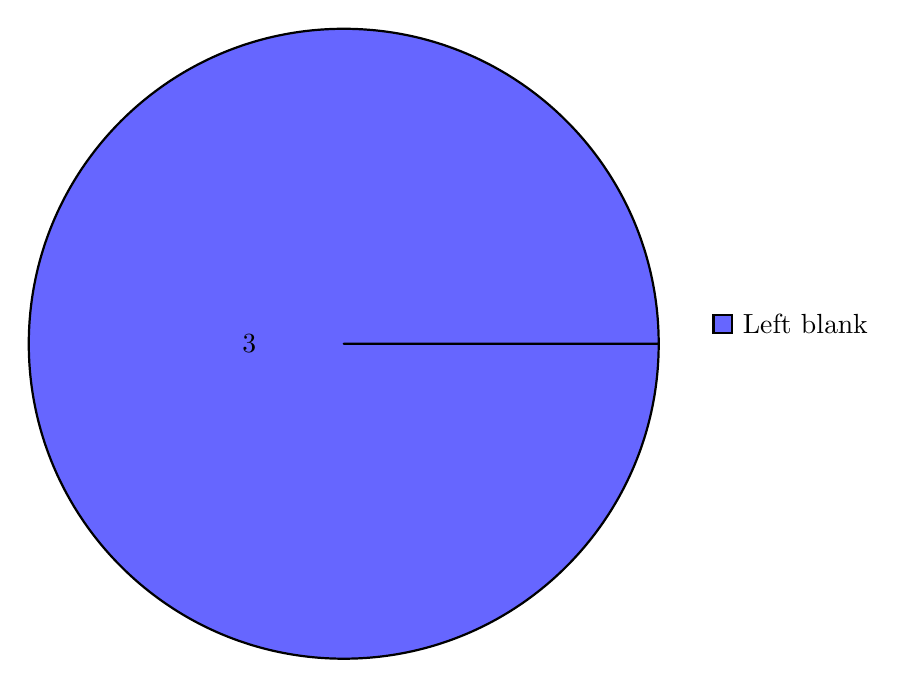
\begin{tikzpicture}
        \pie[radius=4,sum=auto,text=legend]{
            3/Left blank
        }
    \end{tikzpicture}
    \caption{\label{figure:q170-1}Repartition of answers for the question 'IF CONDITION Is Red Lesion 
Location is'.}
\end{figure}



\clearpage{}
\section{Cervical Area
Number of teeth affected}

\label{sec:176}


\begin{figure}[h!]
    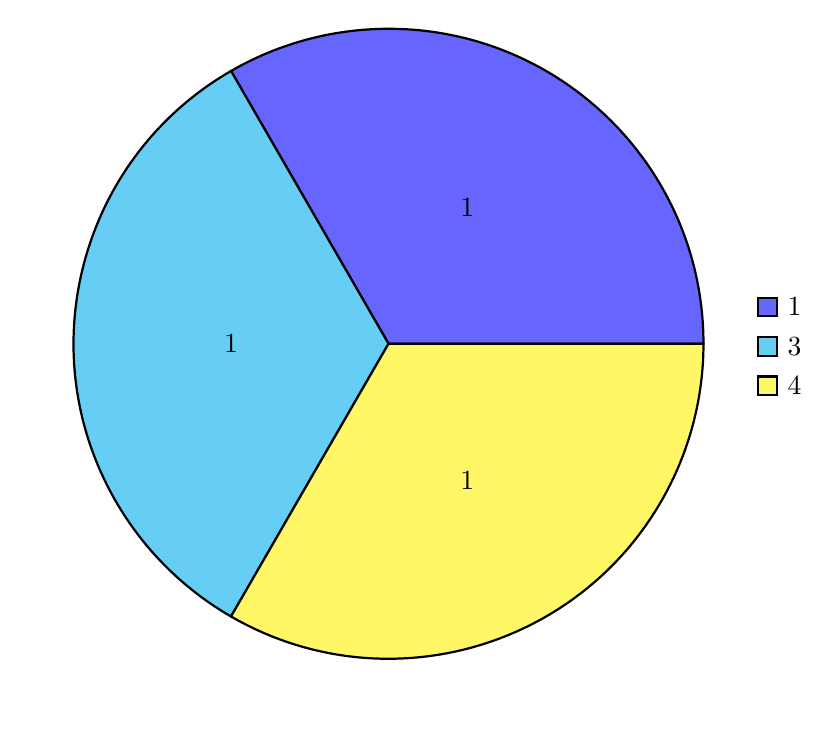
\begin{tikzpicture}
        \pie[radius=4,sum=auto,text=legend]{
            1/1,
            1/3,
            1/4
        }
    \end{tikzpicture}
    \caption{\label{figure:q176-1}Repartition of answers for the question 'Cervical Area
Number of teeth affected'.}
\end{figure}



\clearpage{}
\section{น้ำหนัก}

\label{sec:16}


\begin{figure}[h!]
    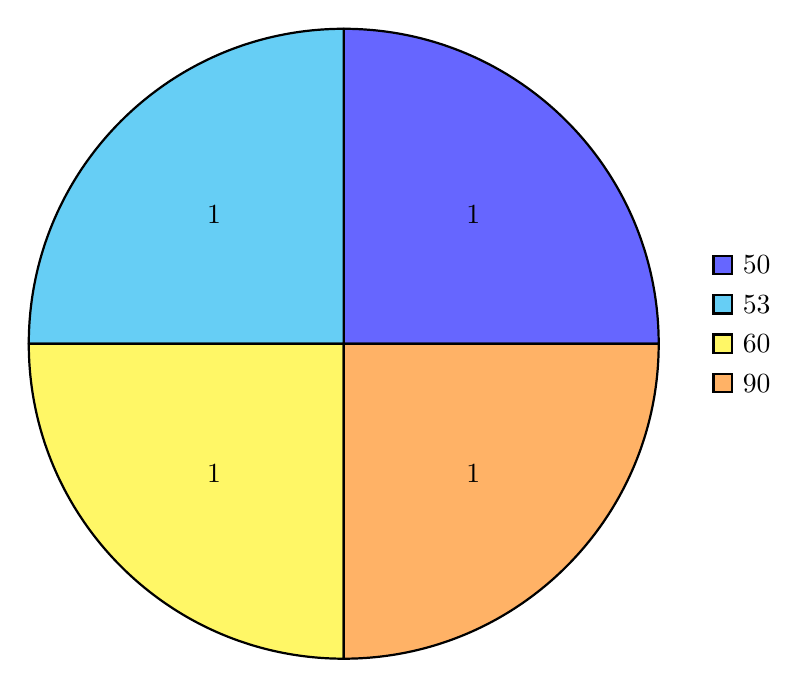
\begin{tikzpicture}
        \pie[radius=4,sum=auto,text=legend]{
            1/50,
            1/53,
            1/60,
            1/90
        }
    \end{tikzpicture}
    \caption{\label{figure:q16-1}Repartition of answers for the question 'น้ำหนัก'.}
\end{figure}



\clearpage{}
\section{15
Crown, Root, Treatment}

\label{sec:28}


\begin{figure}[h!]
    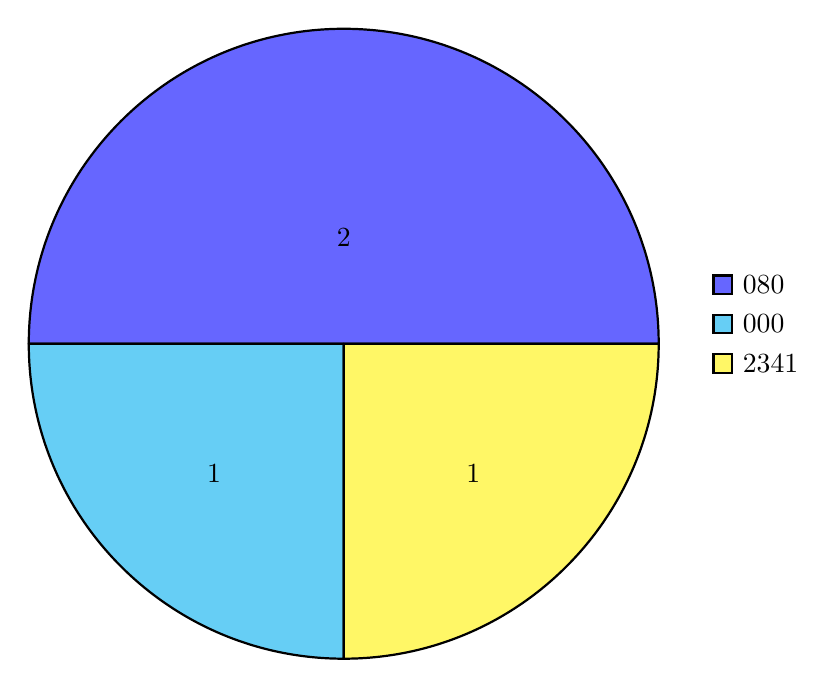
\begin{tikzpicture}
        \pie[radius=4,sum=auto,text=legend]{
            2/080,
            1/000,
            1/2341
        }
    \end{tikzpicture}
    \caption{\label{figure:q28-1}Repartition of answers for the question '15
Crown, Root, Treatment'.}
\end{figure}



\clearpage{}
\section{Gingival Bleeding Scores
47/46 - B}

\label{sec:61}


\begin{figure}[h!]
    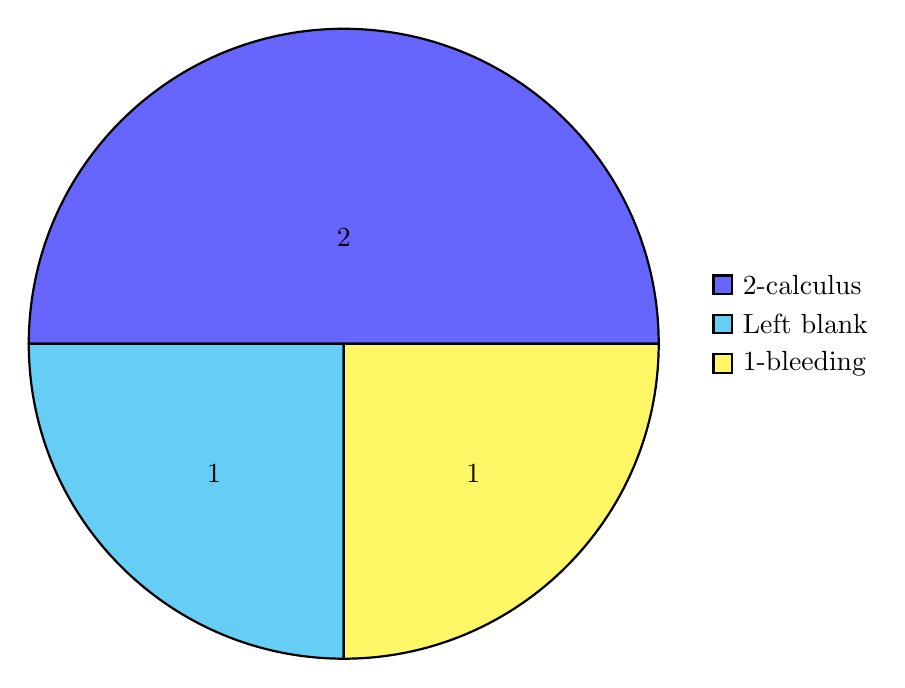
\begin{tikzpicture}
        \pie[radius=4,sum=auto,text=legend]{
            2/2-calculus,
            1/Left blank,
            1/1-bleeding
        }
    \end{tikzpicture}
    \caption{\label{figure:q61-1}Repartition of answers for the question 'Gingival Bleeding Scores
47/46 - B'.}
\end{figure}



\clearpage{}
\section{Prosthetic Need
Lower}

\label{sec:72}


\begin{figure}[h!]
    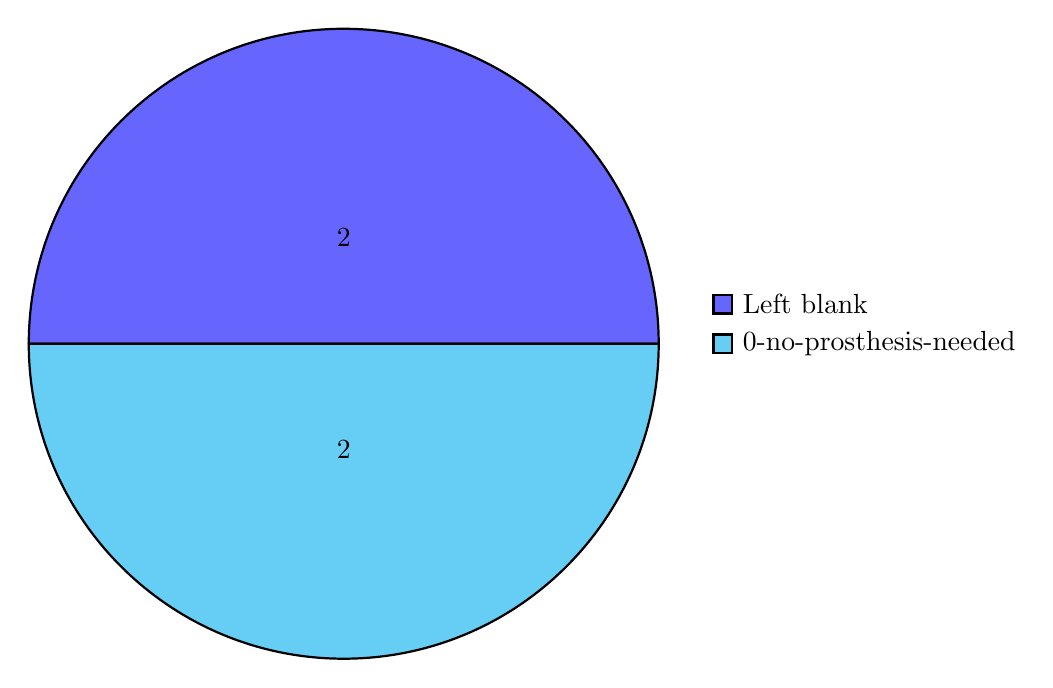
\begin{tikzpicture}
        \pie[radius=4,sum=auto,text=legend]{
            2/Left blank,
            2/0-no-prosthesis-needed
        }
    \end{tikzpicture}
    \caption{\label{figure:q72-1}Repartition of answers for the question 'Prosthetic Need
Lower'.}
\end{figure}



\clearpage{}
\section{IF CONDITION Is Red and White Lesion 
Location is}

\label{sec:171}


\begin{figure}[h!]
    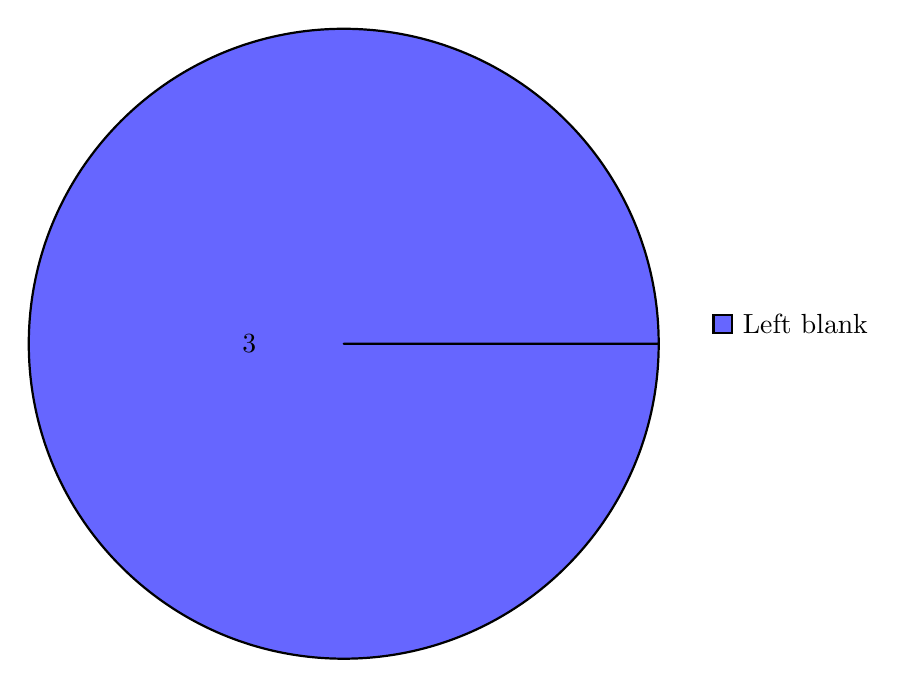
\begin{tikzpicture}
        \pie[radius=4,sum=auto,text=legend]{
            3/Left blank
        }
    \end{tikzpicture}
    \caption{\label{figure:q171-1}Repartition of answers for the question 'IF CONDITION Is Red and White Lesion 
Location is'.}
\end{figure}



\clearpage{}
\section{ส่วนสูง}

\label{sec:17}


\begin{figure}[h!]
    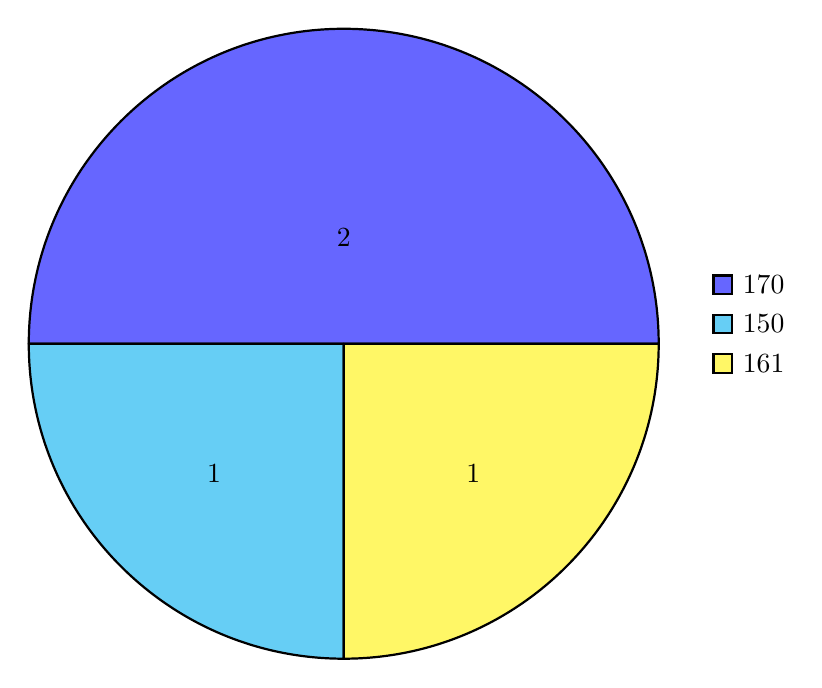
\begin{tikzpicture}
        \pie[radius=4,sum=auto,text=legend]{
            2/170,
            1/150,
            1/161
        }
    \end{tikzpicture}
    \caption{\label{figure:q17-1}Repartition of answers for the question 'ส่วนสูง'.}
\end{figure}



\clearpage{}
\section{14
Crown, Root, Treatment}

\label{sec:29}


\begin{figure}[h!]
    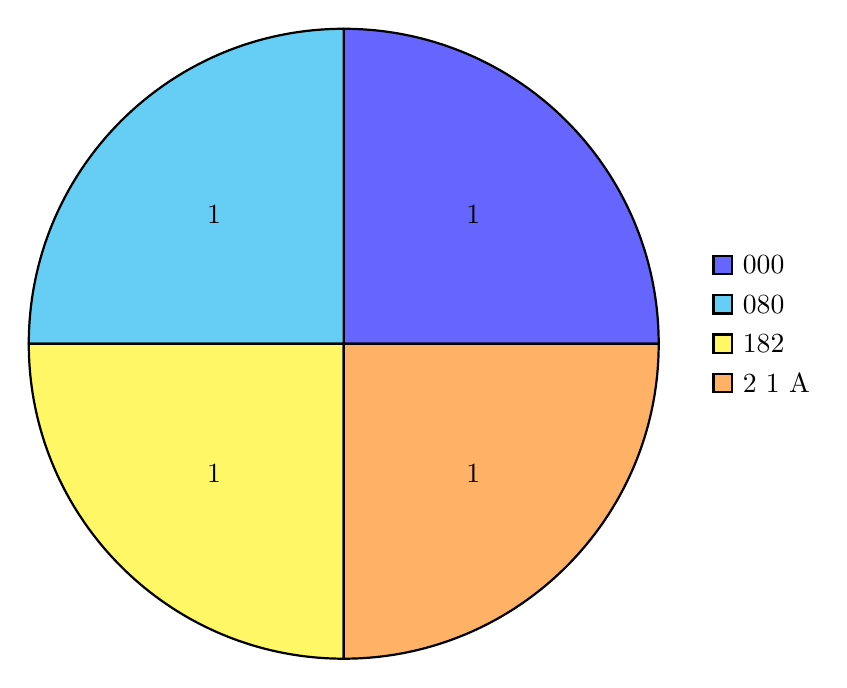
\begin{tikzpicture}
        \pie[radius=4,sum=auto,text=legend]{
            1/000,
            1/080,
            1/182,
            1/2 1 A
        }
    \end{tikzpicture}
    \caption{\label{figure:q29-1}Repartition of answers for the question '14
Crown, Root, Treatment'.}
\end{figure}



\clearpage{}
\section{Gingival Bleeding Scores
31 - B}

\label{sec:62}


\begin{figure}[h!]
    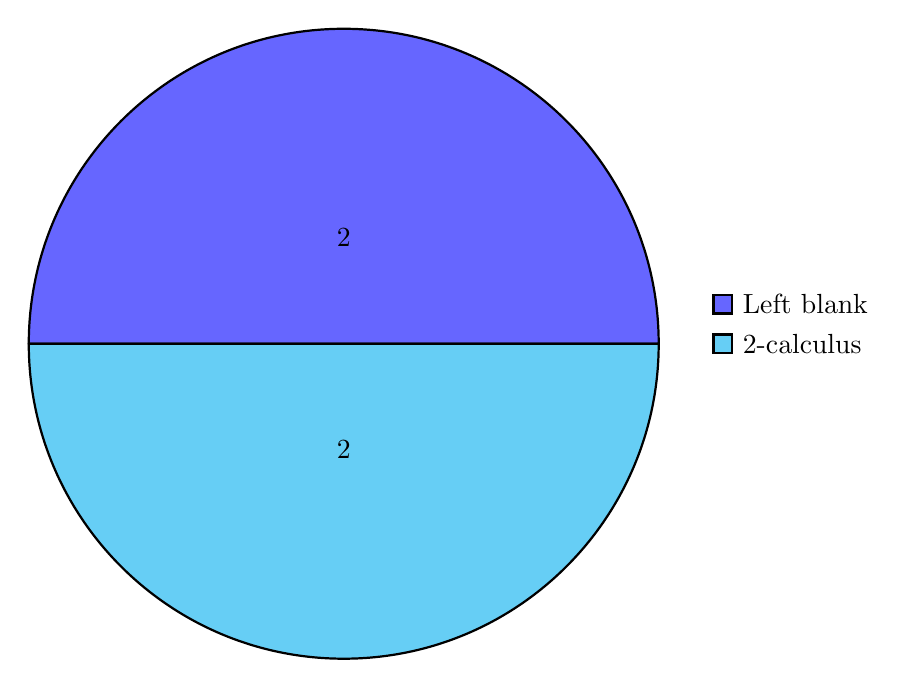
\begin{tikzpicture}
        \pie[radius=4,sum=auto,text=legend]{
            2/Left blank,
            2/2-calculus
        }
    \end{tikzpicture}
    \caption{\label{figure:q62-1}Repartition of answers for the question 'Gingival Bleeding Scores
31 - B'.}
\end{figure}



\clearpage{}
\section{IF CONDITION Is Ulceration
Location is}

\label{sec:172}


\begin{figure}[h!]
    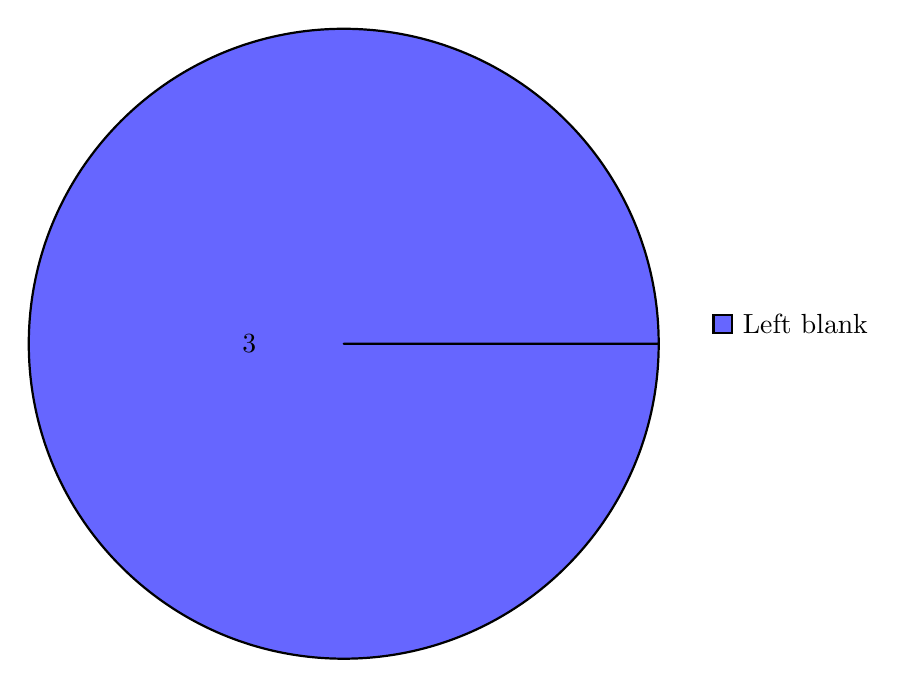
\begin{tikzpicture}
        \pie[radius=4,sum=auto,text=legend]{
            3/Left blank
        }
    \end{tikzpicture}
    \caption{\label{figure:q172-1}Repartition of answers for the question 'IF CONDITION Is Ulceration
Location is'.}
\end{figure}



\clearpage{}
\section{อายุ}

\label{sec:18}


\begin{figure}[h!]
    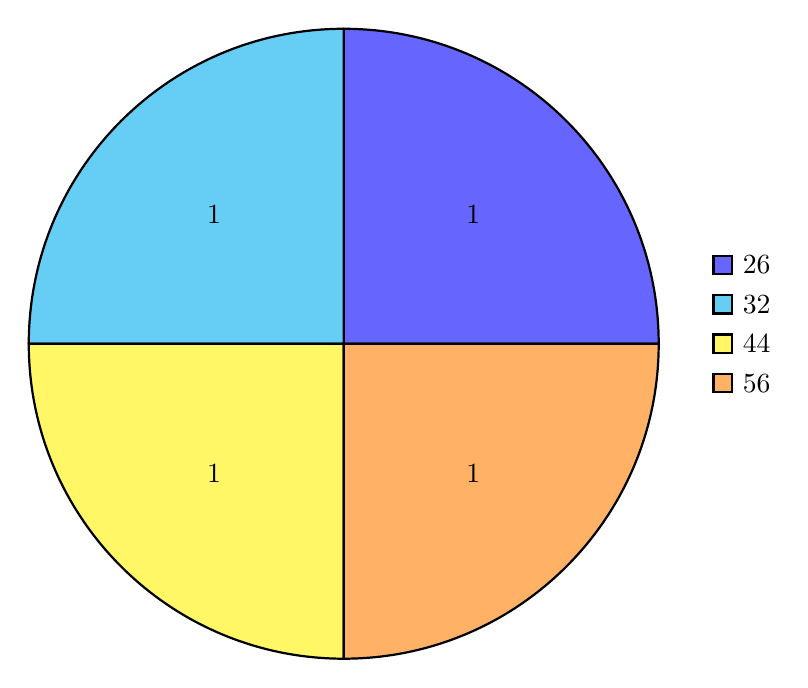
\begin{tikzpicture}
        \pie[radius=4,sum=auto,text=legend]{
            1/26,
            1/32,
            1/44,
            1/56
        }
    \end{tikzpicture}
    \caption{\label{figure:q18-1}Repartition of answers for the question 'อายุ'.}
\end{figure}



\clearpage{}
\section{13
Crown, Root, Treatment}

\label{sec:30}


\begin{figure}[h!]
    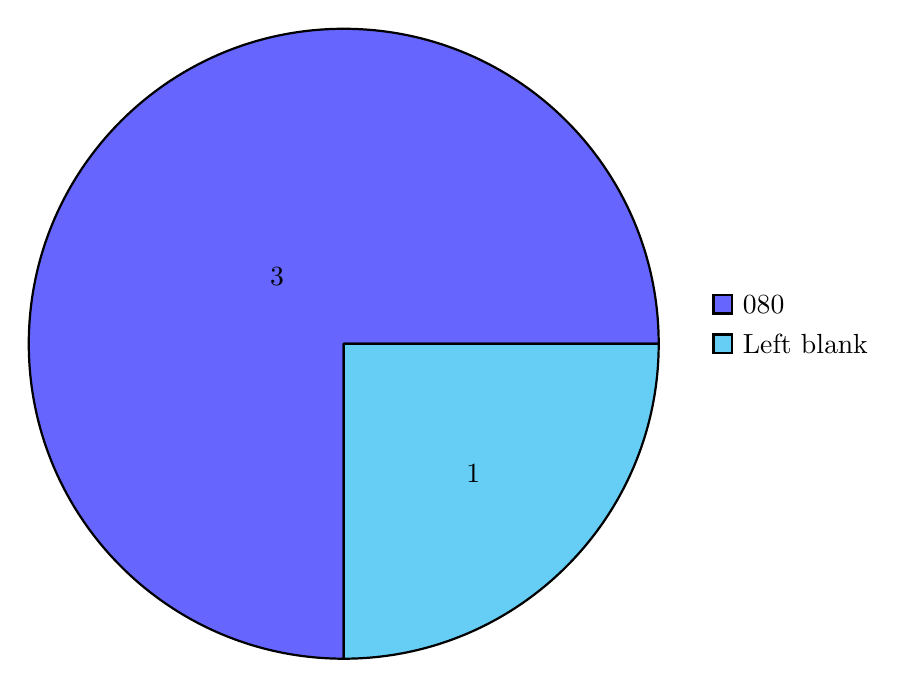
\begin{tikzpicture}
        \pie[radius=4,sum=auto,text=legend]{
            3/080,
            1/Left blank
        }
    \end{tikzpicture}
    \caption{\label{figure:q30-1}Repartition of answers for the question '13
Crown, Root, Treatment'.}
\end{figure}



\clearpage{}
\section{Gingival Bleeding Scores
36/37 - B}

\label{sec:63}


\begin{figure}[h!]
    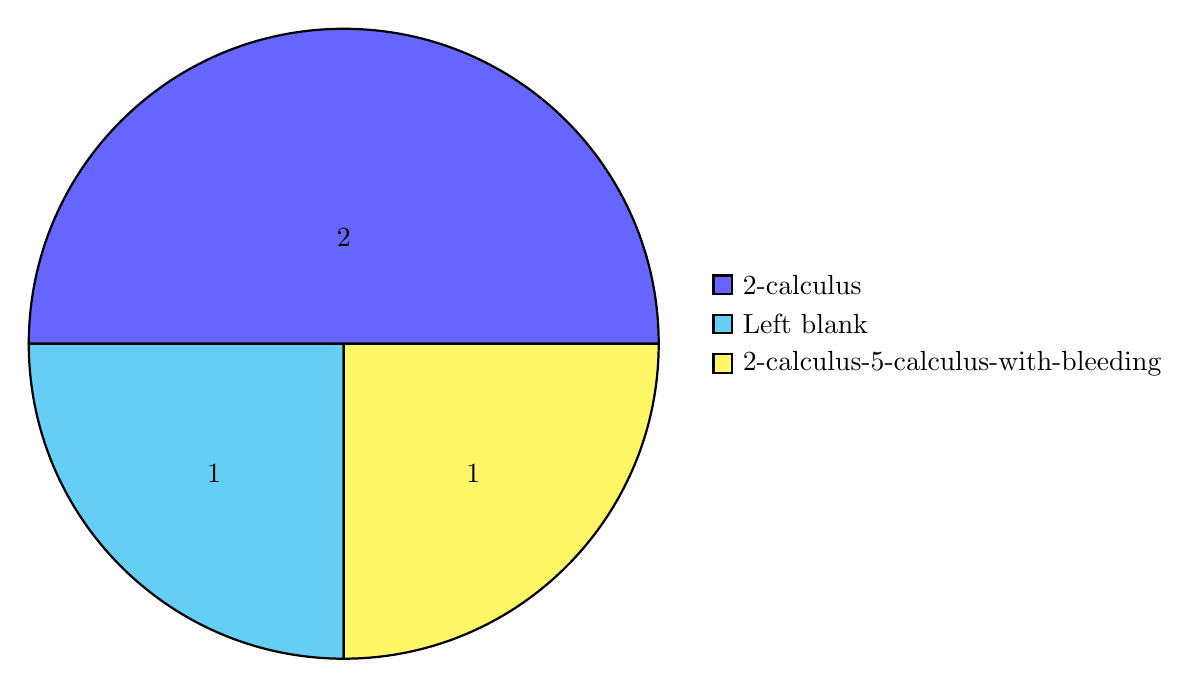
\begin{tikzpicture}
        \pie[radius=4,sum=auto,text=legend]{
            2/2-calculus,
            1/Left blank,
            1/2-calculus-5-calculus-with-bleeding
        }
    \end{tikzpicture}
    \caption{\label{figure:q63-1}Repartition of answers for the question 'Gingival Bleeding Scores
36/37 - B'.}
\end{figure}



\clearpage{}
\section{IF CONDITION Is Nodule/ Mass
Location is}

\label{sec:173}


\begin{figure}[h!]
    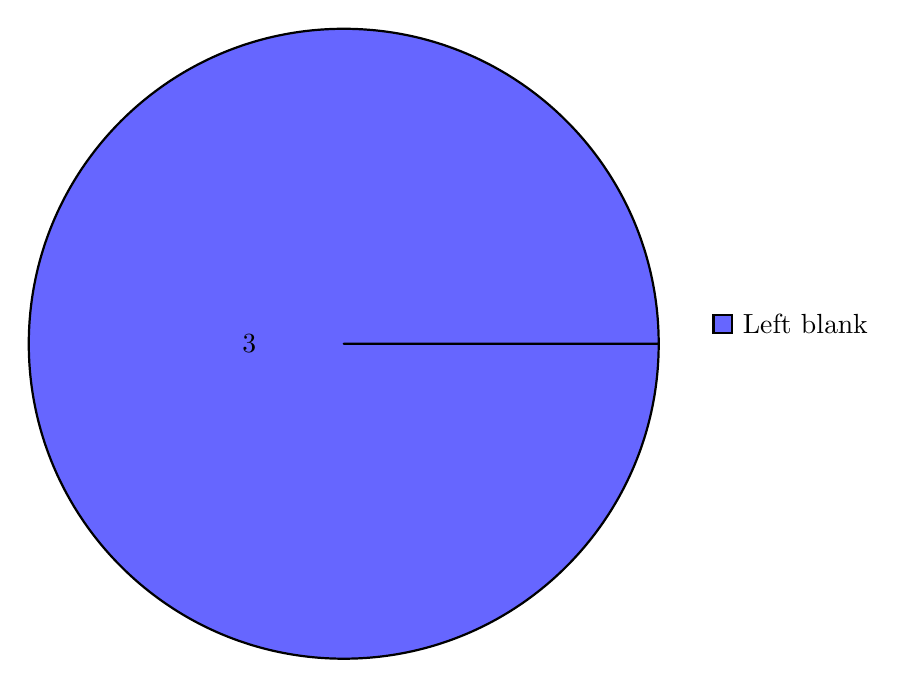
\begin{tikzpicture}
        \pie[radius=4,sum=auto,text=legend]{
            3/Left blank
        }
    \end{tikzpicture}
    \caption{\label{figure:q173-1}Repartition of answers for the question 'IF CONDITION Is Nodule/ Mass
Location is'.}
\end{figure}



\clearpage{}
\section{เพศ}

\label{sec:19}


\begin{figure}[h!]
    \begin{tikzpicture}
        \pie[radius=4,sum=auto,text=legend]{
            3/หญง,
            1/ชาย
        }
    \end{tikzpicture}
    \caption{\label{figure:q19-1}Repartition of answers for the question 'เพศ'.}
\end{figure}



\clearpage{}
\section{12
Crown, Root, Treatment}

\label{sec:31}


\begin{figure}[h!]
    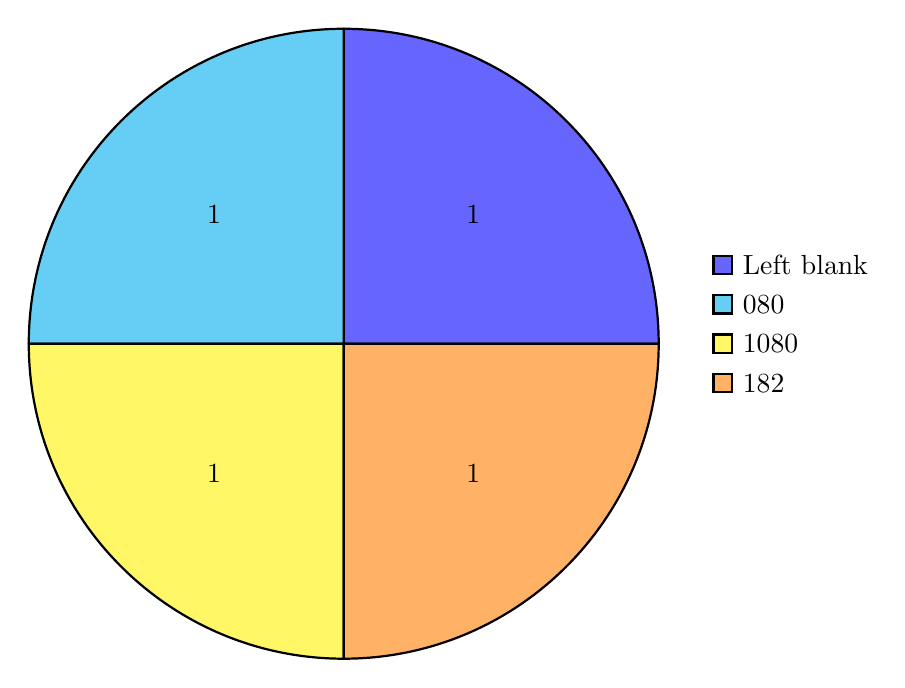
\begin{tikzpicture}
        \pie[radius=4,sum=auto,text=legend]{
            1/Left blank,
            1/080,
            1/1080,
            1/182
        }
    \end{tikzpicture}
    \caption{\label{figure:q31-1}Repartition of answers for the question '12
Crown, Root, Treatment'.}
\end{figure}



\clearpage{}
\section{Pocket Scores
17/16 - P}

\label{sec:58}


\begin{figure}[h!]
    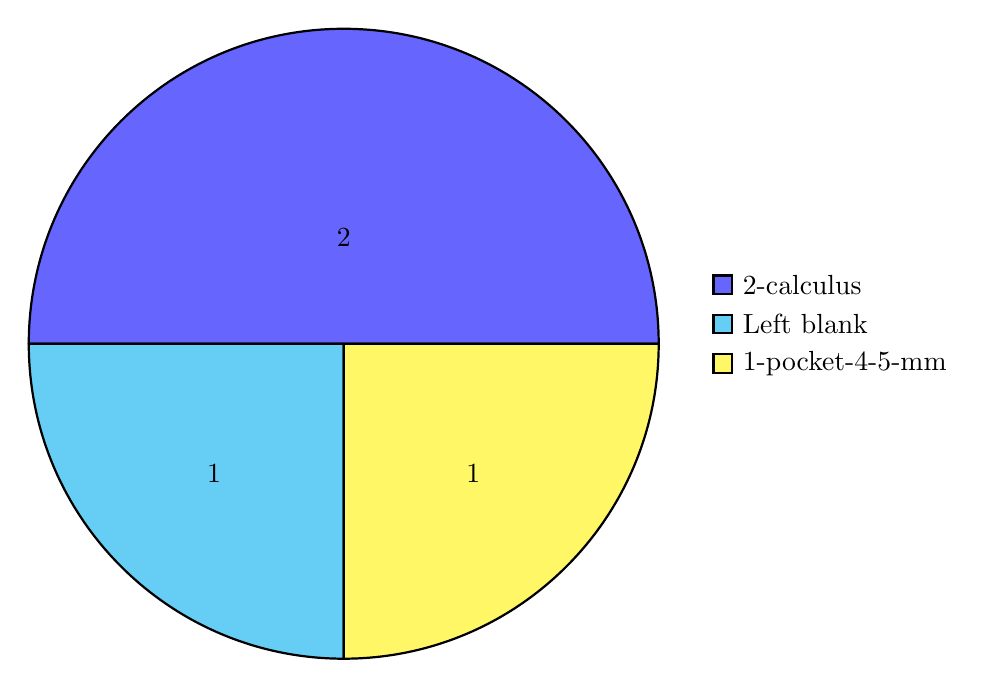
\begin{tikzpicture}
        \pie[radius=4,sum=auto,text=legend]{
            2/2-calculus,
            1/Left blank,
            1/1-pocket-4-5-mm
        }
    \end{tikzpicture}
    \caption{\label{figure:q58-1}Repartition of answers for the question 'Pocket Scores
17/16 - P'.}
\end{figure}



\clearpage{}
\section{Pocket Scores
11 - P}

\label{sec:64}


\begin{figure}[h!]
    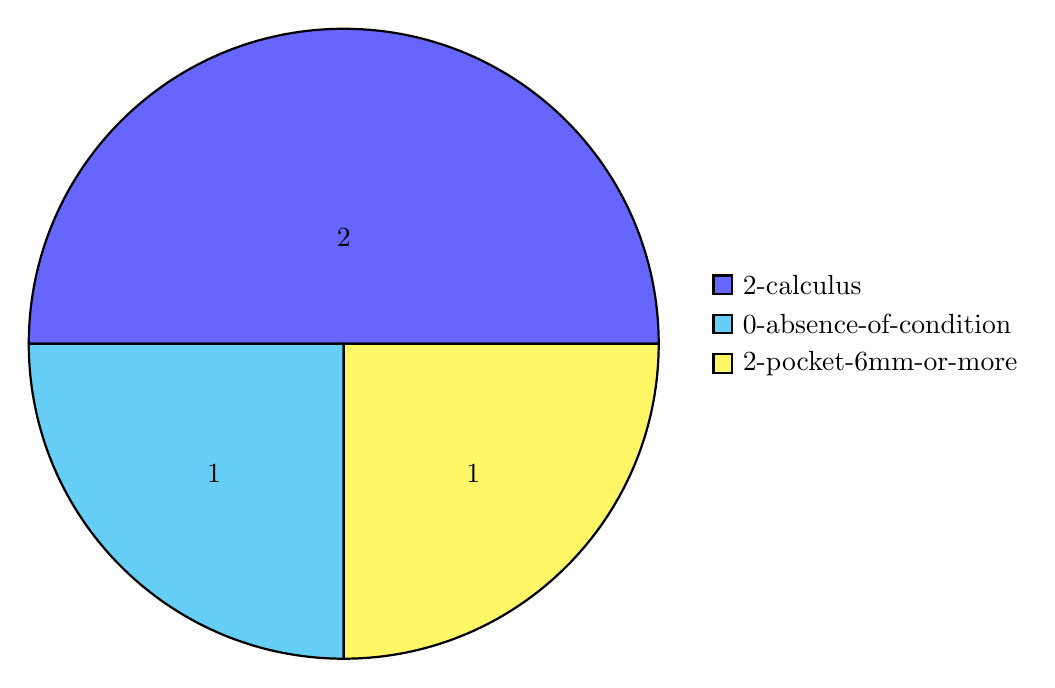
\begin{tikzpicture}
        \pie[radius=4,sum=auto,text=legend]{
            2/2-calculus,
            1/0-absence-of-condition,
            1/2-pocket-6mm-or-more
        }
    \end{tikzpicture}
    \caption{\label{figure:q64-1}Repartition of answers for the question 'Pocket Scores
11 - P'.}
\end{figure}



\clearpage{}
\section{ศาสนา}

\label{sec:20}


\begin{figure}[h!]
    \begin{tikzpicture}
        \pie[radius=4,sum=auto,text=legend]{
            3/พทธ,
            1/ครสต
        }
    \end{tikzpicture}
    \caption{\label{figure:q20-1}Repartition of answers for the question 'ศาสนา'.}
\end{figure}



\clearpage{}
\section{11
Crown, Root, Treatment}

\label{sec:32}


\begin{figure}[h!]
    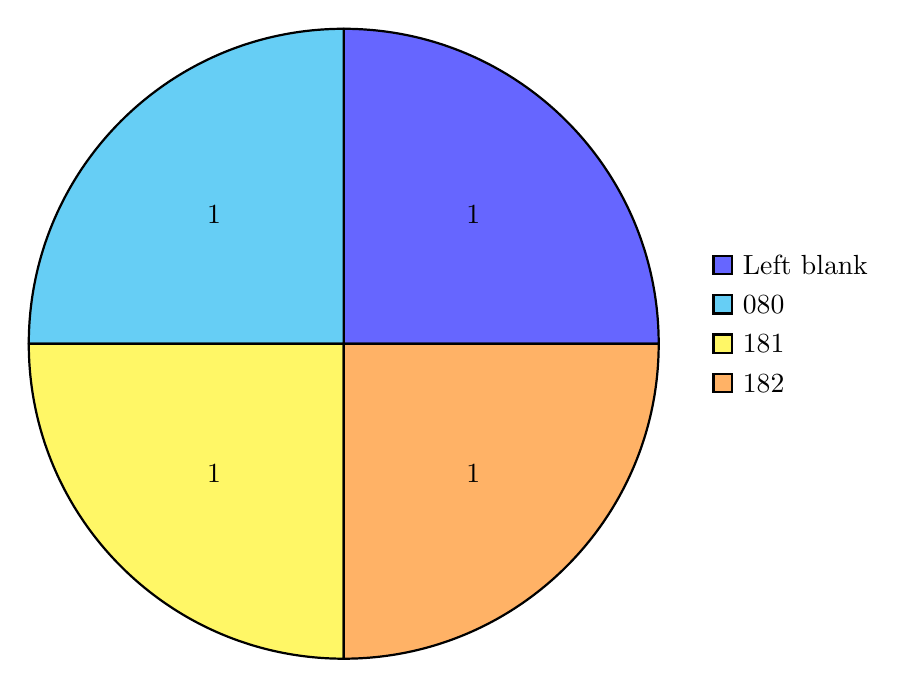
\begin{tikzpicture}
        \pie[radius=4,sum=auto,text=legend]{
            1/Left blank,
            1/080,
            1/181,
            1/182
        }
    \end{tikzpicture}
    \caption{\label{figure:q32-1}Repartition of answers for the question '11
Crown, Root, Treatment'.}
\end{figure}



\clearpage{}
\section{Pocket Scores
26/27 - P}

\label{sec:65}


\begin{figure}[h!]
    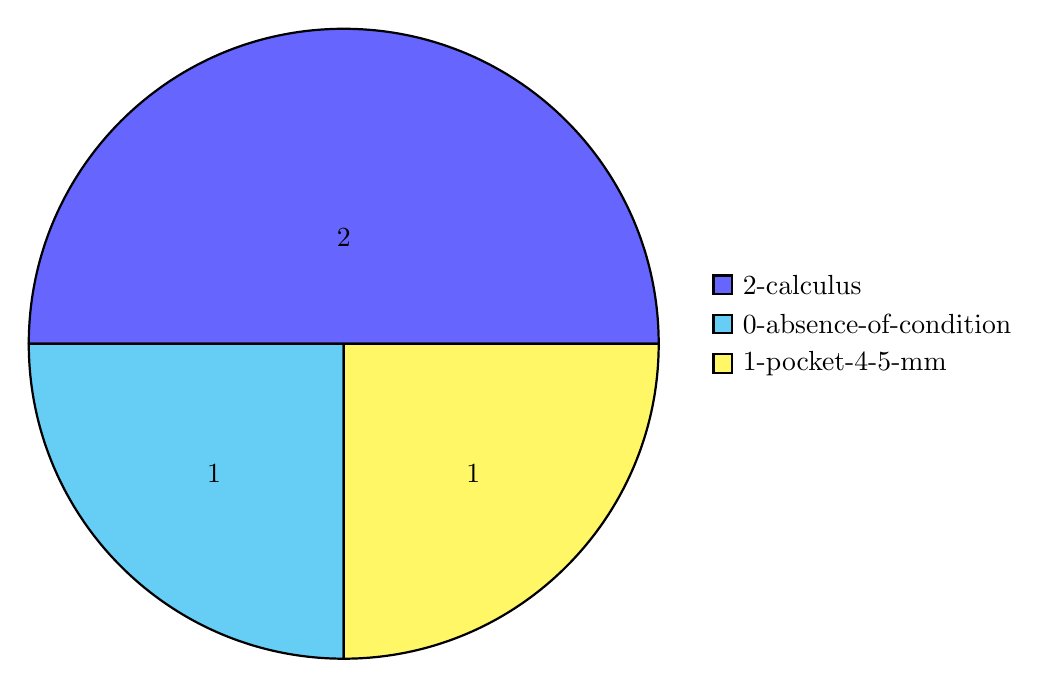
\begin{tikzpicture}
        \pie[radius=4,sum=auto,text=legend]{
            2/2-calculus,
            1/0-absence-of-condition,
            1/1-pocket-4-5-mm
        }
    \end{tikzpicture}
    \caption{\label{figure:q65-1}Repartition of answers for the question 'Pocket Scores
26/27 - P'.}
\end{figure}



\clearpage{}
\section{การศึกษา}

\label{sec:21}


\begin{figure}[h!]
    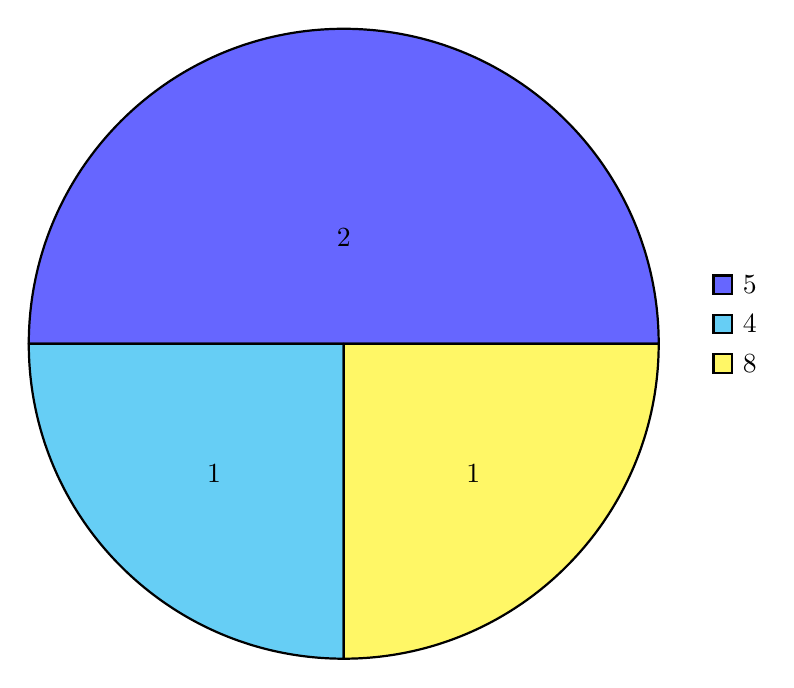
\begin{tikzpicture}
        \pie[radius=4,sum=auto,text=legend]{
            2/5,
            1/4,
            1/8
        }
    \end{tikzpicture}
    \caption{\label{figure:q21-1}Repartition of answers for the question 'การศึกษา'.}
\end{figure}



\clearpage{}
\section{Capacity of old adults}

\label{sec:22}


\begin{figure}[h!]
    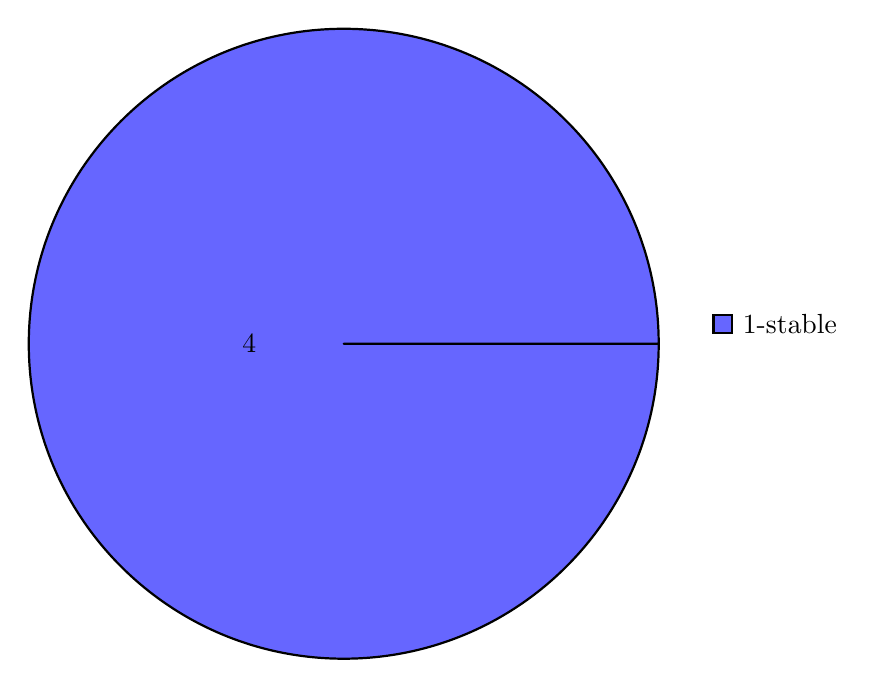
\begin{tikzpicture}
        \pie[radius=4,sum=auto,text=legend]{
            4/1-stable
        }
    \end{tikzpicture}
    \caption{\label{figure:q22-1}Repartition of answers for the question 'Capacity of old adults'.}
\end{figure}



\clearpage{}
\section{21
Crown, Root, Treatment}

\label{sec:33}


\begin{figure}[h!]
    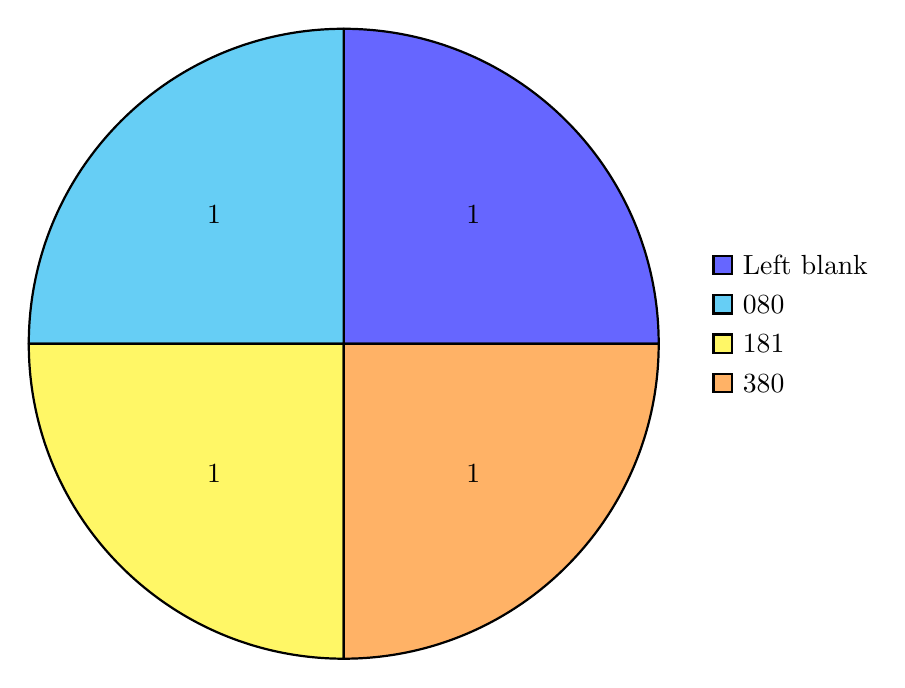
\begin{tikzpicture}
        \pie[radius=4,sum=auto,text=legend]{
            1/Left blank,
            1/080,
            1/181,
            1/380
        }
    \end{tikzpicture}
    \caption{\label{figure:q33-1}Repartition of answers for the question '21
Crown, Root, Treatment'.}
\end{figure}



\clearpage{}
\section{Pocket Scores
47/46 - P}

\label{sec:66}


\begin{figure}[h!]
    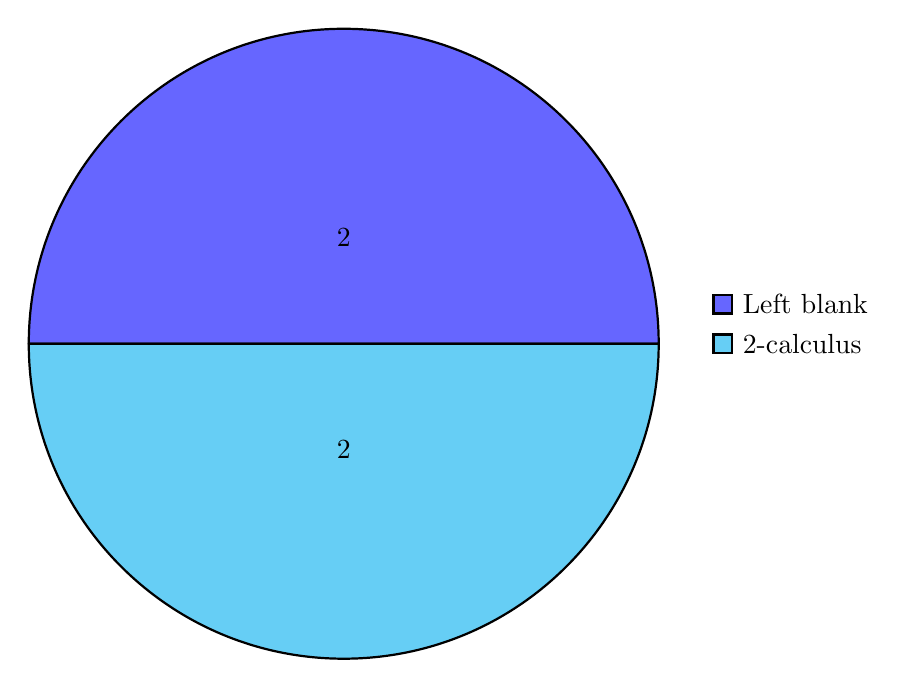
\begin{tikzpicture}
        \pie[radius=4,sum=auto,text=legend]{
            2/Left blank,
            2/2-calculus
        }
    \end{tikzpicture}
    \caption{\label{figure:q66-1}Repartition of answers for the question 'Pocket Scores
47/46 - P'.}
\end{figure}



\clearpage{}
\section{22
Crown, Root, Treatment}

\label{sec:34}


\begin{figure}[h!]
    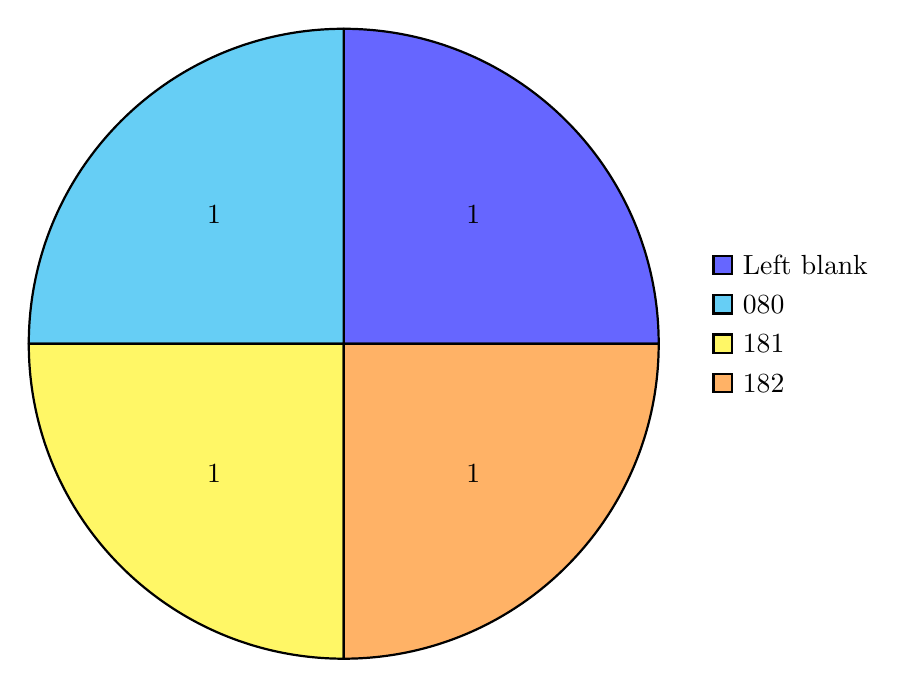
\begin{tikzpicture}
        \pie[radius=4,sum=auto,text=legend]{
            1/Left blank,
            1/080,
            1/181,
            1/182
        }
    \end{tikzpicture}
    \caption{\label{figure:q34-1}Repartition of answers for the question '22
Crown, Root, Treatment'.}
\end{figure}



\clearpage{}
\section{Pocket Scores
31 - P}

\label{sec:67}


\begin{figure}[h!]
    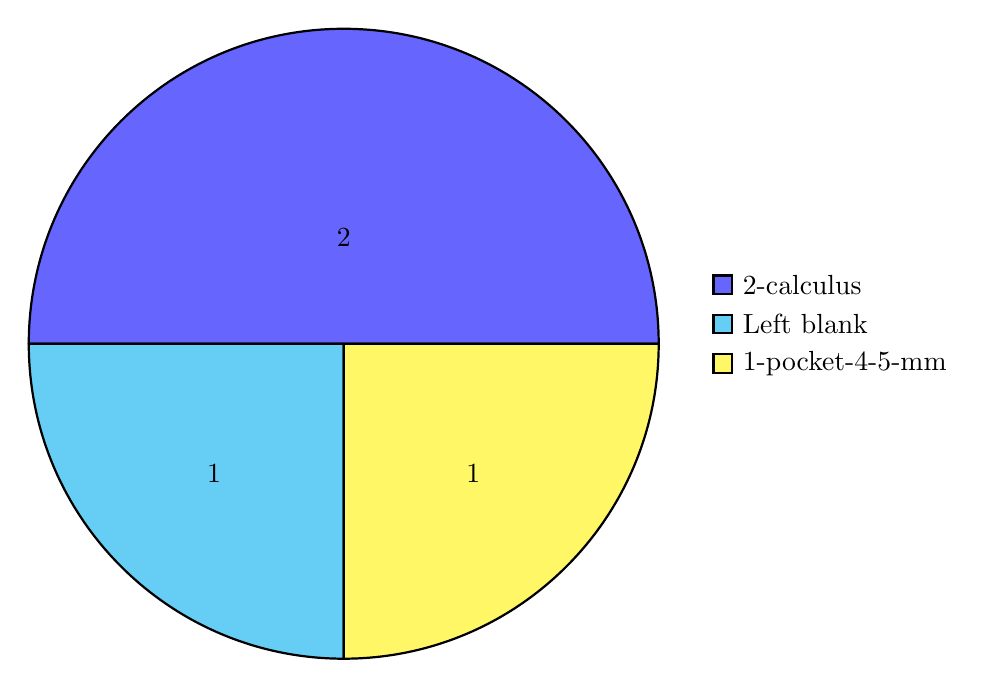
\begin{tikzpicture}
        \pie[radius=4,sum=auto,text=legend]{
            2/2-calculus,
            1/Left blank,
            1/1-pocket-4-5-mm
        }
    \end{tikzpicture}
    \caption{\label{figure:q67-1}Repartition of answers for the question 'Pocket Scores
31 - P'.}
\end{figure}



\clearpage{}
\section{23
Crown, Root, Treatment}

\label{sec:35}


\begin{figure}[h!]
    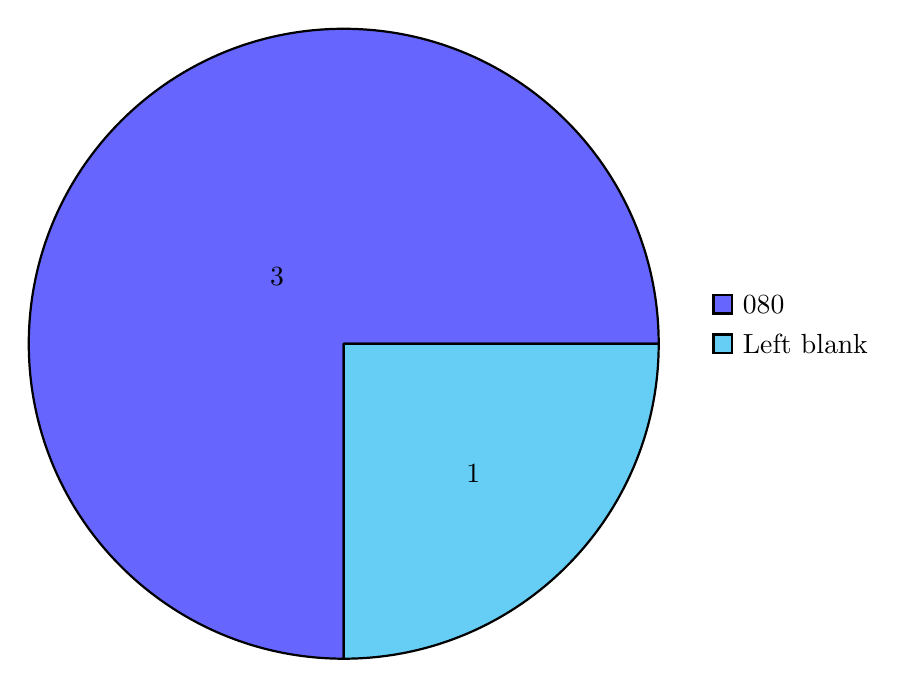
\begin{tikzpicture}
        \pie[radius=4,sum=auto,text=legend]{
            3/080,
            1/Left blank
        }
    \end{tikzpicture}
    \caption{\label{figure:q35-1}Repartition of answers for the question '23
Crown, Root, Treatment'.}
\end{figure}



\clearpage{}
\section{Pocket Scores
36/37 - P}

\label{sec:68}


\begin{figure}[h!]
    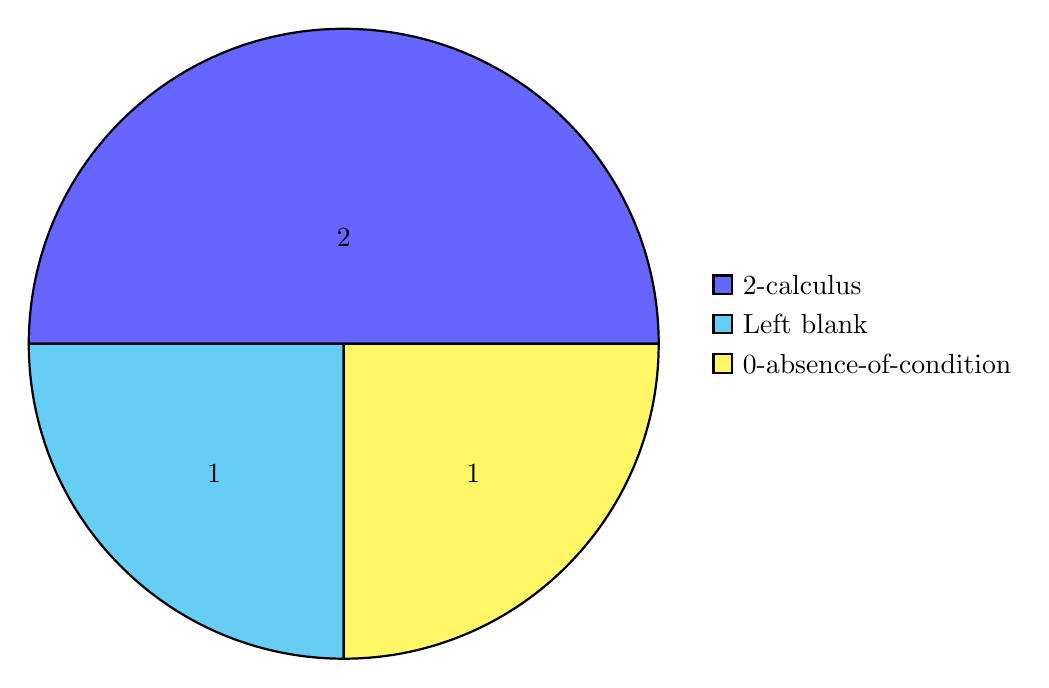
\begin{tikzpicture}
        \pie[radius=4,sum=auto,text=legend]{
            2/2-calculus,
            1/Left blank,
            1/0-absence-of-condition
        }
    \end{tikzpicture}
    \caption{\label{figure:q68-1}Repartition of answers for the question 'Pocket Scores
36/37 - P'.}
\end{figure}



\clearpage{}
\section{24
Crown, Root, Treatment}

\label{sec:36}


\begin{figure}[h!]
    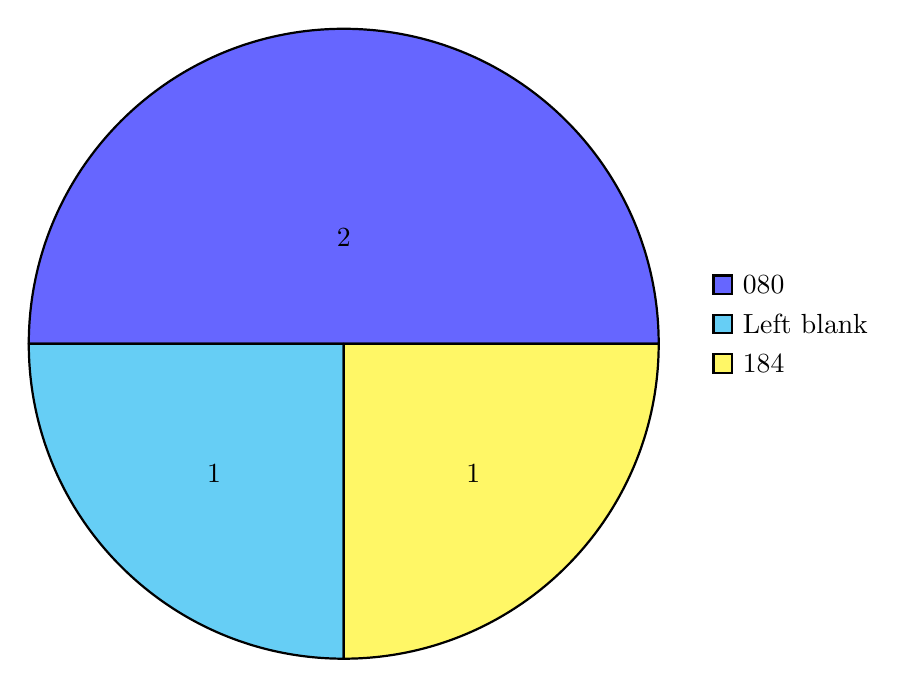
\begin{tikzpicture}
        \pie[radius=4,sum=auto,text=legend]{
            2/080,
            1/Left blank,
            1/184
        }
    \end{tikzpicture}
    \caption{\label{figure:q36-1}Repartition of answers for the question '24
Crown, Root, Treatment'.}
\end{figure}



\clearpage{}
\section{25
Crown, Root, Treatment}

\label{sec:37}


\begin{figure}[h!]
    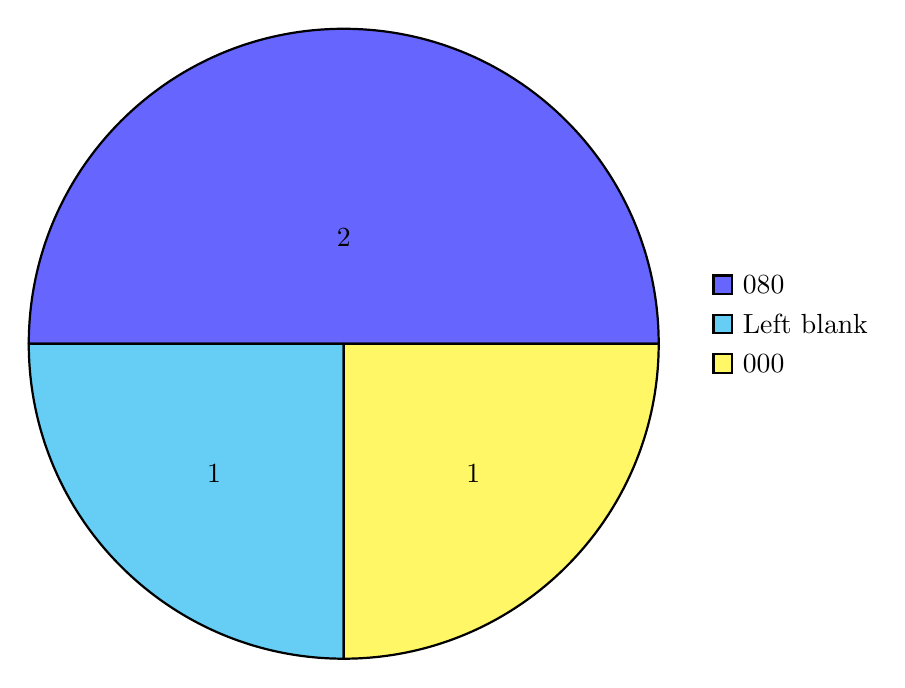
\begin{tikzpicture}
        \pie[radius=4,sum=auto,text=legend]{
            2/080,
            1/Left blank,
            1/000
        }
    \end{tikzpicture}
    \caption{\label{figure:q37-1}Repartition of answers for the question '25
Crown, Root, Treatment'.}
\end{figure}



\clearpage{}
\section{26
Crown, Root, Treatment}

\label{sec:38}


\begin{figure}[h!]
    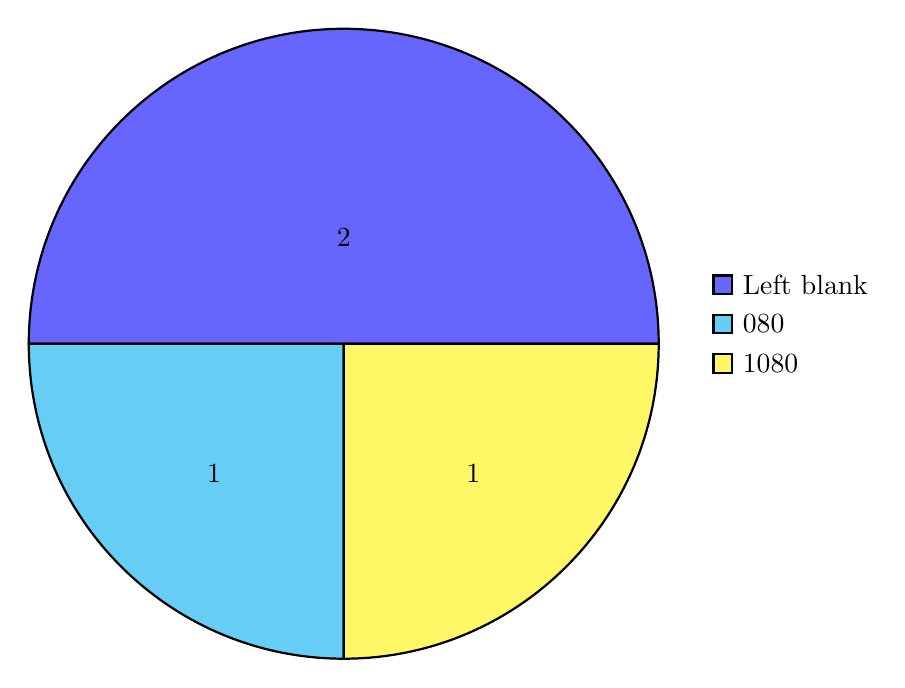
\begin{tikzpicture}
        \pie[radius=4,sum=auto,text=legend]{
            2/Left blank,
            1/080,
            1/1080
        }
    \end{tikzpicture}
    \caption{\label{figure:q38-1}Repartition of answers for the question '26
Crown, Root, Treatment'.}
\end{figure}



\clearpage{}
\section{27
Crown, Root, Treatment}

\label{sec:39}


\begin{figure}[h!]
    \begin{tikzpicture}
        \pie[radius=4,sum=auto,text=legend]{
            2/Left blank,
            1/080,
            1/180
        }
    \end{tikzpicture}
    \caption{\label{figure:q39-1}Repartition of answers for the question '27
Crown, Root, Treatment'.}
\end{figure}



\clearpage{}
\section{28
Crown, Root, Treatment}

\label{sec:40}


\begin{figure}[h!]
    \begin{tikzpicture}
        \pie[radius=4,sum=auto,text=legend]{
            1/Left blank,
            1/180,
            1/182,
            1/380
        }
    \end{tikzpicture}
    \caption{\label{figure:q40-1}Repartition of answers for the question '28
Crown, Root, Treatment'.}
\end{figure}



\clearpage{}
\section{38
Crown, Root, Treatment}

\label{sec:56}


\begin{figure}[h!]
    \begin{tikzpicture}
        \pie[radius=4,sum=auto,text=legend]{
            2/Left blank,
            1/182,
            1/995
        }
    \end{tikzpicture}
    \caption{\label{figure:q56-1}Repartition of answers for the question '38
Crown, Root, Treatment'.}
\end{figure}



\clearpage{}
\section{37
Crown, Root, Treatment}

\label{sec:55}


\begin{figure}[h!]
    \begin{tikzpicture}
        \pie[radius=4,sum=auto,text=legend]{
            2/Left blank,
            1/080,
            1/184
        }
    \end{tikzpicture}
    \caption{\label{figure:q55-1}Repartition of answers for the question '37
Crown, Root, Treatment'.}
\end{figure}



\clearpage{}
\section{36
Crown, Root, Treatment}

\label{sec:54}


\begin{figure}[h!]
    \begin{tikzpicture}
        \pie[radius=4,sum=auto,text=legend]{
            2/Left blank,
            1/080,
            1/280
        }
    \end{tikzpicture}
    \caption{\label{figure:q54-1}Repartition of answers for the question '36
Crown, Root, Treatment'.}
\end{figure}



\clearpage{}
\section{35
Crown, Root, Treatment}

\label{sec:53}


\begin{figure}[h!]
    \begin{tikzpicture}
        \pie[radius=4,sum=auto,text=legend]{
            2/Left blank,
            2/080
        }
    \end{tikzpicture}
    \caption{\label{figure:q53-1}Repartition of answers for the question '35
Crown, Root, Treatment'.}
\end{figure}



\clearpage{}
\section{34
Crown, Root, Treatment}

\label{sec:52}


\begin{figure}[h!]
    \begin{tikzpicture}
        \pie[radius=4,sum=auto,text=legend]{
            2/Left blank,
            2/080
        }
    \end{tikzpicture}
    \caption{\label{figure:q52-1}Repartition of answers for the question '34
Crown, Root, Treatment'.}
\end{figure}



\clearpage{}
\section{33
Crown, Root, Treatment}

\label{sec:51}


\begin{figure}[h!]
    \begin{tikzpicture}
        \pie[radius=4,sum=auto,text=legend]{
            2/Left blank,
            2/080
        }
    \end{tikzpicture}
    \caption{\label{figure:q51-1}Repartition of answers for the question '33
Crown, Root, Treatment'.}
\end{figure}



\clearpage{}
\section{32
Crown, Root, Treatment}

\label{sec:50}


\begin{figure}[h!]
    \begin{tikzpicture}
        \pie[radius=4,sum=auto,text=legend]{
            2/Left blank,
            2/080
        }
    \end{tikzpicture}
    \caption{\label{figure:q50-1}Repartition of answers for the question '32
Crown, Root, Treatment'.}
\end{figure}



\clearpage{}
\section{31
Crown, Root, Treatment}

\label{sec:49}


\begin{figure}[h!]
    \begin{tikzpicture}
        \pie[radius=4,sum=auto,text=legend]{
            2/080,
            1/Left blank,
            1/599
        }
    \end{tikzpicture}
    \caption{\label{figure:q49-1}Repartition of answers for the question '31
Crown, Root, Treatment'.}
\end{figure}



\clearpage{}
\section{41
Crown, Root, Treatment}

\label{sec:48}


\begin{figure}[h!]
    \begin{tikzpicture}
        \pie[radius=4,sum=auto,text=legend]{
            2/Left blank,
            2/080
        }
    \end{tikzpicture}
    \caption{\label{figure:q48-1}Repartition of answers for the question '41
Crown, Root, Treatment'.}
\end{figure}



\clearpage{}
\section{42
Crown, Root, Treatment}

\label{sec:47}


\begin{figure}[h!]
    \begin{tikzpicture}
        \pie[radius=4,sum=auto,text=legend]{
            2/080,
            1/Left blank,
            1/000
        }
    \end{tikzpicture}
    \caption{\label{figure:q47-1}Repartition of answers for the question '42
Crown, Root, Treatment'.}
\end{figure}



\clearpage{}
\section{43
Crown, Root, Treatment}

\label{sec:46}


\begin{figure}[h!]
    \begin{tikzpicture}
        \pie[radius=4,sum=auto,text=legend]{
            3/080,
            1/Left blank
        }
    \end{tikzpicture}
    \caption{\label{figure:q46-1}Repartition of answers for the question '43
Crown, Root, Treatment'.}
\end{figure}



\clearpage{}
\section{44
Crown, Root, Treatment}

\label{sec:45}


\begin{figure}[h!]
    \begin{tikzpicture}
        \pie[radius=4,sum=auto,text=legend]{
            3/080,
            1/Left blank
        }
    \end{tikzpicture}
    \caption{\label{figure:q45-1}Repartition of answers for the question '44
Crown, Root, Treatment'.}
\end{figure}



\clearpage{}
\section{45
Crown, Root, Treatment}

\label{sec:44}


\begin{figure}[h!]
    \begin{tikzpicture}
        \pie[radius=4,sum=auto,text=legend]{
            2/080,
            1/Left blank,
            1/599
        }
    \end{tikzpicture}
    \caption{\label{figure:q44-1}Repartition of answers for the question '45
Crown, Root, Treatment'.}
\end{figure}



\clearpage{}
\section{46
Crown, Root, Treatment}

\label{sec:43}


\begin{figure}[h!]
    \begin{tikzpicture}
        \pie[radius=4,sum=auto,text=legend]{
            2/080,
            1/Left blank,
            1/1080
        }
    \end{tikzpicture}
    \caption{\label{figure:q43-1}Repartition of answers for the question '46
Crown, Root, Treatment'.}
\end{figure}



\clearpage{}
\section{47
Crown, Root, Treatment}

\label{sec:42}


\begin{figure}[h!]
    \begin{tikzpicture}
        \pie[radius=4,sum=auto,text=legend]{
            1/Left blank,
            1/180,
            1/181,
            1/380
        }
    \end{tikzpicture}
    \caption{\label{figure:q42-1}Repartition of answers for the question '47
Crown, Root, Treatment'.}
\end{figure}



\clearpage{}
\section{48
Crown, Root, Treatment}

\label{sec:41}


\begin{figure}[h!]
    \begin{tikzpicture}
        \pie[radius=4,sum=auto,text=legend]{
            2/Left blank,
            1/185,
            1/995
        }
    \end{tikzpicture}
    \caption{\label{figure:q41-1}Repartition of answers for the question '48
Crown, Root, Treatment'.}
\end{figure}



\end{document}
